%% ----------------------------------------------------------------
%% Thesis.tex -- MAIN FILE (the one that you compile with LaTeX)
%% ---------------------------------------------------------------- 

% Set up the document
\documentclass[a4paper, 11pt, oneside]{Thesis}  % Use the "Thesis" style, based on the ECS Thesis style by Steve Gunn
\graphicspath{Figures/}  % Location of the graphics files (set up for graphics to be in PDF format)

% Include any extra LaTeX packages required
\usepackage[square, numbers, comma, sort&compress]{natbib}  % Use the "Natbib" style for the references in the Bibliography
\usepackage{verbatim}  % Needed for the "comment" environment to make LaTeX comments
\usepackage{vector}  % Allows "\bvec{}" and "\buvec{}" for "blackboard" style bold vectors in maths
\usepackage{algorithm}
\usepackage{algorithmicx}
\usepackage{algpseudocode}
\usepackage{url}
\usepackage{hyperref}
\hypersetup{urlcolor=blue, colorlinks=true}  % Colours hyperlinks in blue, but this can be distracting if there are many links.

\usepackage{listings}
\usepackage{color} %red, green, blue, yellow, cyan, magenta, black, white
\definecolor{mygreen}{RGB}{28,172,0} % color values Red, Green, Blue
\definecolor{mylilas}{RGB}{170,55,241}

\lstset{language=Matlab,%
    breaklines=true,%
    morekeywords={matlab2tikz},
    keywordstyle=\color{blue},%
    morekeywords=[2]{1}, keywordstyle=[2]{\color{black}},
    identifierstyle=\color{black},%
    stringstyle=\color{mylilas},
    commentstyle=\color{mygreen},%
    showstringspaces=false,%without this there will be a symbol in the places where there is a space
    emph=[1]{for,end,break},emphstyle=[1]\color{red}, %some words to emphasise
    %emph=[2]{word1,word2}, emphstyle=[2]{style},    
}

% Python style for highlighting
\newcommand\pythonstyle{\lstset{
language=Python,
basicstyle=\ttm,
otherkeywords={self},             % Add keywords here
keywordstyle=\ttb\color{deepblue},
emph={MyClass,__init__},          % Custom highlighting
emphstyle=\ttb\color{deepred},    % Custom highlighting style
stringstyle=\color{deepgreen},
frame=tb,                         % Any extra options here
showstringspaces=false            % 
}}

%% ----------------------------------------------------------------
\begin{document}
\frontmatter      % Begin Roman style (i, ii, iii, iv...) page numbering

% Set up the Title Page
\title {Techniques for Fault Detection and Visualization of Telemetry Dependence Relationships for Root Cause Fault Analysis in Complex Systems}
\authors  {\texorpdfstring
            {\href{natguy@uw.edu}{Nathaniel Guy}}
            {Nathaniel Guy}
            }
\addresses  {\groupname\\\deptname\\\univname}  % Do not change this here, instead these must be set in the "Thesis.cls" file, please look through it instead
\date       {\today}
\subject    {}
\keywords   {}

\maketitle
%% ----------------------------------------------------------------

\setstretch{1.3}  % It is better to have smaller font and larger line spacing than the other way round

% Define the page headers using the FancyHdr package and set up for one-sided printing
\fancyhead{}  % Clears all page headers and footers
\rhead{\thepage}  % Sets the right side header to show the page number
\lhead{}  % Clears the left side page header

\pagestyle{fancy}  % Finally, use the "fancy" page style to implement the FancyHdr headers

%% ----------------------------------------------------------------
% Declaration Page required for the Thesis, your institution may give you a different text to place here
\Declaration{

\addtocontents{toc}{\vspace{1em}}  % Add a gap in the Contents, for aesthetics

I, NATHANIEL GUY, declare that this thesis titled, `TECHNIQUES FOR FAULT DETECTION AND VISUALIZATION OF TELEMETRY DEPENDENCE RELATIONSHIPS FOR ROOT CAUSE FAULT ANALYSIS IN COMPLEX SYSTEMS' and the work presented in it are my own. I confirm that:

\begin{itemize} 
\item[\tiny{$\blacksquare$}] This work was done wholly or mainly while in candidature for a research degree at this University.
 
\item[\tiny{$\blacksquare$}] Where any part of this thesis has previously been submitted for a degree or any other qualification at this University or any other institution, this has been clearly stated.
 
\item[\tiny{$\blacksquare$}] Where I have consulted the published work of others, this is always clearly attributed.
 
\item[\tiny{$\blacksquare$}] Where I have quoted from the work of others, the source is always given. With the exception of such quotations, this thesis is entirely my own work.
 
\item[\tiny{$\blacksquare$}] I have acknowledged all main sources of help.
 
\item[\tiny{$\blacksquare$}] Where the thesis is based on work done by myself jointly with others, I have made clear exactly what was done by others and what I have contributed myself.
\\
\end{itemize}
 
Signed:\\
\rule[1em]{25em}{0.5pt}  % This prints a line for the signature
 
Date:\\
\rule[1em]{25em}{0.5pt}  % This prints a line to write the date
}
\clearpage  % Declaration ended, now start a new page

%% ----------------------------------------------------------------
\pagestyle{empty}  % No headers or footers for the following pages

\null\vfill
\textit{``Okay, 13. We've got lots and lots of people working on this; we'll give you some dope as soon
as we have it, and you'll be the first one to know.'}

\begin{flushright}
Jack Lousma, Apollo 13 CapCom \cite{apollo13}
\end{flushright}

\vfill\vfill\vfill\vfill\vfill\vfill\null
\clearpage  % Funny Quote page ended, start a new page
%% ----------------------------------------------------------------

% The Abstract Page
\addtotoc{Abstract}  % Add the "Abstract" page entry to the Contents
\abstract{
\addtocontents{toc}{\vspace{1em}}  % Add a gap in the Contents, for aesthetics

This thesis explores new ways of looking at telemetry data, from a time-correlative perspective, in order to see patterns within the data that may suggest root causes of system faults. It was thought initially that visualizing an animated Pearson Correlation Coefficient (PCC) matrix for telemetry channels would be sufficient to give new understanding; however, testing showed that the high dimensionality and inability to easily look at change over time in this approach impeded understanding. Different correlative techniques, combined with the time curve visualization proposed by Bach et al (2015), were adapted to visualize both raw telemetry and telemetry data correlations. Review revealed insights into understanding and an intuitive grasp of data families that suggests the viability of this approach to enhance system understanding root cause analysis for actual aerospace systems.

}

\clearpage  % Abstract ended, start a new page
%% ----------------------------------------------------------------

\setstretch{1.3}  % Reset the line-spacing to 1.3 for body text (if it has changed)

% The Acknowledgements page, for thanking everyone
\acknowledgements{
\addtocontents{toc}{\vspace{1em}}  % Add a gap in the Contents, for aesthetics

I would like to thank my advisor, Dr. Mehran Mesbahi, for his academic guidance, his patience, and his constant encouragement as I struggled with the process of determining my own interests in this field. Deep thanks go to Dr. Jeff Heer for his insights and suggestions into the best practices for visualizing the hidden patterns within correlation data. My sincere thanks to Dr. Chris Lum for his opinions and suggestions about aerospace fault detection systems. I'd also like thank my various internship teams for their guidance and encouragement: the JPL OpsLab team, specifically Scott Davidoff, Jeff Norris, and Garrett Johnson, for introducing me to teleoperation interface design and testing techniques with the Unity 3D game engine; the SpaceX Flight Software team, specifically Mike Soares, Dan Gelband and Derek Bronish, for introducing me to Fault Detection, Isolation and Recovery systems and teaching me much about aerospace ground software systems; and the HAKUTO Lunar XPRIZE team, specifically Dr. Nathan Britton, Louis Burtz, Toshiro ``Dark" Shimizu, Toshiki Tanaka, Dr. John Walker, and Dr. Kazuya Yoshida for letting me use their lunar rover as a testbed for new ground software design methodologies and fault diagnosis techniques, and for their friendship and support. Special thanks go to Daisuke Kikuchi for countless bits of design advice and for helping to increase the aesthetic appeal of the HAKUTO rover ground station UI. My thanks to the team at Unity, for developing an excellent and adaptive game engine. Finally, I'd like to thank Steve Rabin at Nintendo of America for his advice about fault detection and valuable comparisons to runtime analysis and profiling of executable code. Without the aforementioned people and many others, I would be lost!

}
\clearpage  % End of the Acknowledgements
%% ----------------------------------------------------------------

\pagestyle{fancy}  %The page style headers have been "empty" all this time, now use the "fancy" headers as defined before to bring them back


%% ----------------------------------------------------------------
\lhead{\emph{Contents}}  % Set the left side page header to "Contents"
\tableofcontents  % Write out the Table of Contents

%% ----------------------------------------------------------------
\lhead{\emph{List of Figures}}  % Set the left side page header to "List if Figures"
\listoffigures  % Write out the List of Figures

%% ----------------------------------------------------------------
\lhead{\emph{List of Tables}}  % Set the left side page header to "List of Tables"
\listoftables  % Write out the List of Tables

%% ----------------------------------------------------------------
\setstretch{1.5}  % Set the line spacing to 1.5, this makes the following tables easier to read
\clearpage  % Start a new page
\lhead{\emph{Abbreviations}}  % Set the left side page header to "Abbreviations"
\listofsymbols{ll}  % Include a list of Abbreviations (a table of two columns)
{
% \textbf{Acronym} & \textbf{W}hat (it) \textbf{S}tands \textbf{F}or \\
\textbf{FD} & \textbf{F}ault \textbf{D}etection \\
\textbf{FDIR} & \textbf{F}ault \textbf{D}etection, \textbf{I}solation, and \textbf{R}ecovery \\
\textbf{GSN} & \textbf{G}round \textbf{S}tatio\textbf{n} \\
\textbf{IMU} & \textbf{I}nertial \textbf{M}easurement \textbf{U}nit \\
\textbf{JAXA} & \textbf{J}apanese \textbf{A}erospace e\textbf{X}ploration \textbf{A}gency \\
\textbf{PCA} & \textbf{P}rincipal \textbf{C}omponent \textbf{A}nalysis \\
\textbf{PCC} & \textbf{P}earson \textbf{C}orrelation \textbf{C}oefficient \\
\textbf{SRL} & \textbf{S}pace \textbf{R}obotics \textbf{L}aboratory \\
\textbf{SVD} & \textbf{S}ingular \textbf{V}alue \textbf{D}ecomposition \\

}

%% ----------------------------------------------------------------
%\clearpage  % Start a new page
%\lhead{\emph{Physical Constants}}  % Set the left side page header to "Physical Constants"
%\listofconstants{lrcl}  % Include a list of Physical Constants (a four column table)
%{
%% Constant Name & Symbol & = & Constant Value (with units) \\
%Speed of Light & $c$ & $=$ & $2.997\ 924\ 58\times10^{8}\ \mbox{ms}^{-\mbox{s}}$ (exact)\\
%
%}

%% ----------------------------------------------------------------
\clearpage  %Start a new page
\lhead{\emph{Symbols}}  % Set the left side page header to "Symbols"
\listofnomenclature{lll}  % Include a list of Symbols (a three column table)
{
% symbol & name & unit \\
$\rho_{X, Y}$ & Spearman's Rho Correlation Coefficient for variables $X$ and $Y$ &  \\
$\tau_{X, Y}$ & Kendall's Tau Correlation Coefficient for variables $X$ and $Y$ &  \\
$D$ & Distance matrix (for state differences) & \\
$C$ & Correlation matrix & \\
$C_{all}$ & Horizontally stacked matrix of flattened correlation matrices at each time step & \\
$D_{ij}$ & Row $i$, column $j$ of $D$ & \\
$D_{i, :}$ & Row $i$, all columns of $D$ & \\
$M$ & State history matrix & \\
$r_{PCC, X, Y}$ & Pearson's Correlation Coefficient for variables $X$ and $Y$ &  \\
$t$ & Time; number of time steps & \\
$w$ & Window size & \\
$W$ & Windowed sample matrix (a subset of the state history matrix) &  \\

& & \\ % Gap to separate the Roman symbols from the Greek
%$\omega$ & angular frequency & rads$^{-1}$ \\
}
%% ----------------------------------------------------------------
% End of the preamble, contents and lists of things
% Begin the Dedication page

\setstretch{1.3}  % Return the line spacing back to 1.3
\lhead{}  % Clears the left side page header

\pagestyle{empty}  % Page style needs to be empty for this page
\dedicatory{For Carl, who showed me the way to space.}

\addtocontents{toc}{\vspace{2em}}  % Add a gap in the Contents, for aesthetics


%% ----------------------------------------------------------------
\mainmatter	  % Begin normal, numeric (1,2,3...) page numbering
\pagestyle{fancy}  % Return the page headers back to the "fancy" style

% Include the chapters of the thesis, as separate files
% Just uncomment the lines as you write the chapters

\chapter{Introduction}

Complex, remote-operated systems present many problems to engineers and designers who are conscious of mission safety. Complex systems often have detailed and comprehensive rules for the detection of anomalous conditions, or ``faults," but even the most complex cannot capture the full range of possible anomalies that can occur on a system, especially if false positives are a concern and if the designers have not thought of all possible conditions. Visualization of fault conditions can be an even greater problem, owing to issues such as the impracticality of simultaneously displaying data from thousands of telemetry channels, organizing data in a logical and discoverable way, maintaining system reliability in the presence of performance constraints, and leaving screen space for other non-fault-related visualization components and control affordances.

Because of these difficulties, root cause analysis can be a very long and difficult task. There are several historical cases of major system anomalies that have required very long periods of concentrated, manual telemetry data analysis (and, in some of the most catastrophic cases, post-disassembly hardware analysis) in order to piece together the root cause for anomalies. Some examples include:

\begin{itemize}

\item On October 28th, 2014, the Orbital Sciences ``Antares" rocket suffered a catastrophic failure 6 seconds after launch, experiencing a large explosion which destroyed its cargo, which had been bound for the International Space Station. Orbital Sciences immediately launched an investigation to determine the cause, but preliminary root cause data loosely linking the mishap to a failure of one of the AJ26 engines was not publicly indicated until November 5th, and a final root cause assessment has still not, to this date, been released \cite{spaceflight_antares}. An independent review team within NASA evaluated telemetry data, historical data and hardware samples, beginning in November 2014, and roughly a year later, issued a report that was still unable to provide a clear root cause for the mishap, instead linking it to three likely causes, all involving the AJ26 engine which initially exploded \cite{nasa_orb3}.

\item On July 28th, 2015, SpaceX's ``Falcon 9" rocket, carrying the ``CRS-7" payload delivery up to the International Space Station, experienced an overpressure event in the second stage liquid oxygen tank, causing rapid unscheduled disassembly and failure of the mission. SpaceX engineers, working with NASA and the Air Force, began intensively examining system telemetry from the event. Despite SpaceX's well-known history of transparency about anomalous events and engineering challenges, the root cause of a flawed second-stage helium system strut was not publicly identified until nearly a month later, on July 20th \cite{spacex_crs7}.

\item On December 4th, 2015, the PROCYON interplanetary cubesat, developed by the University of Tokyo and JAXA, went completely ``dark," ceasing to provide any telemetry data at all. As of March of 2016, attempts to analyze previously received telemetry data in order to gain insight into the cause of the anomaly, and possible ideas for recovery, continue, but no root cause has been able to be determined \cite{procyon_status}.

\end{itemize}

As is shown by the cases above, the root cause diagnosis process is very difficult, and can take weeks to months to complete. It involves intense scrutiny of potentially thousands of data channels, and often the only comprehensive understanding of how these data channels relate to each other is encoded in human ``tribal knowledge." Although the examples above are extreme ones, root cause diagnosis can be extremely valuable even with trivial anomalies for gaining a better understanding of system properties and subsystem connections, and the tools to do so that are currently in use are inadequate for the task. Having seen this problem first-hand in the space industry, we set out to examine the space of possible tools that could begin to tackle this problem.

In this thesis, we will examine some possible solutions to the long-standing problem of root cause analysis for complex, remotely monitored systems. The thesis starts with a review of schemes for identification of irregular telemetry via a typical fault detection models, and describes the necessity to characterize anomalous conditions in a more in-depth way than traditional fault detection algorithms allow, in order to identify root causes for anomalies, or to predict the occurrence of anomalous conditions ahead of time. We will point out some of the issues that commonly occur with time series data on multiple channels which can make it difficult to both analyze and visualize.

Next, we will examine traditional methods of analyzing connections between sets of time series data. We will see how solutions to some of the aforementioned issues are provided by these analytical techniques. We will also examine a number of visualization techniques that have been used in the past to show connections within correlation data.

We will propose a data visualization technique, based on an animated adaptation of statistical correlation matrices. To assess the efficacy of this visualization, we will apply it to simulated data from a sample system, and will show test results when users are given an implementation of this visualization and asked to use it to gain insight into events during a simulated scenario. We will discuss some of the downsides of our techniques that were uncovered by testing.

Next, we will iterate and propose adaptations to address some of the issues in the first round of testing. We will look at analytical improvements as well as new visualizations, borrowing from recent research in the field of temporal data visualization, and will evaluate them for their efficacy.

Finally, we will present our conclusions about the employed analysis and visualization techniques, and will propose avenues for further research. % Introduction

\chapter{Background in Fault Detection, Isolation and Recovery}

Purpose:

-lay out some basic fd theory
-get some equations out there
-talk about thresholding and residuals and mathematical models
-explain how faults are limited in what they can capture
-talk about some solutions to this, like learning models
-talk about their downsides, like needing to have a lot of training data, and hardness to debug
-lead into the higher-level analysis of correlation between faults, and my theories about how this can be effective

There is a rich body of literature related to telemetry visualization techniques and fault diagnosis. We borrowed insight and several visualization techniques from the literature. Cancro et al. developed useful techniques for packing large numbers of channels into a dense rectangular space \cite{Cancro}, and Yairi et al. demonstrated ways to show change correlation between data channels \cite{Yairi}, which were inspirations for our Global Correlation Matrix and Channel Correlation Vector. Simple fault detection methodology was adapted from Willsky \cite{Willsky}.


\section{A Section}

Quisque tristique urna in lorem laoreet at laoreet quam congue. Donec dolor turpis, blandit non imperdiet aliquet, blandit et felis. In lorem nisi, pretium sit amet vestibulum sed, tempus et sem. Proin non ante turpis. Nulla imperdiet fringilla convallis. Vivamus vel bibendum nisl. Pellentesque justo lectus, molestie vel luctus sed, lobortis in libero. Nulla facilisi. Aliquam erat volutpat. Suspendisse vitae nunc nunc. Sed aliquet est suscipit sapien rhoncus non adipiscing nibh consequat. Aliquam metus urna, faucibus eu vulputate non, luctus eu justo.

\subsection{A Subsection}

Donec urna leo, vulputate vitae porta eu, vehicula blandit libero. Phasellus eget massa et leo condimentum mollis. Nullam molestie, justo at pellentesque vulputate, sapien velit ornare diam, nec gravida lacus augue non diam. Integer mattis lacus id libero ultrices sit amet mollis neque molestie. Integer ut leo eget mi volutpat congue. Vivamus sodales, turpis id venenatis placerat, tellus purus adipiscing magna, eu aliquam nibh dolor id nibh. Pellentesque habitant morbi tristique senectus et netus et malesuada fames ac turpis egestas. Sed cursus convallis quam nec vehicula. Sed vulputate neque eget odio fringilla ac sodales urna feugiat.

\section{Another Section}

Phasellus nisi quam, volutpat non ullamcorper eget, congue fringilla leo. Cras et erat et nibh placerat commodo id ornare est. Nulla facilisi. Aenean pulvinar scelerisque eros eget interdum. Nunc pulvinar magna ut felis varius in hendrerit dolor accumsan. Nunc pellentesque magna quis magna bibendum non laoreet erat tincidunt. Nulla facilisi.

Duis eget massa sem, gravida interdum ipsum. Nulla nunc nisl, hendrerit sit amet commodo vel, varius id tellus. Lorem ipsum dolor sit amet, consectetur adipiscing elit. Nunc ac dolor est. Suspendisse ultrices tincidunt metus eget accumsan. Nullam facilisis, justo vitae convallis sollicitudin, eros augue malesuada metus, nec sagittis diam nibh ut sapien. Duis blandit lectus vitae lorem aliquam nec euismod nisi volutpat. Vestibulum ornare dictum tortor, at faucibus justo tempor non. Nulla facilisi. Cras non massa nunc, eget euismod purus. Nunc metus ipsum, euismod a consectetur vel, hendrerit nec nunc. % Background in Fault Detection, Isolation and Recovery

\chapter{Correlative Analysis and Visualization}

The chapter looks at some of the fundamentals of correlative analysis for dynamic systems, and discusses the merits and demerits of various correlative methods. We also look at historical techniques that have been used to visualize such data, and propose a visualization variant to capture changing correlation data over time.

\section{Correlation for Fault Analysis: Motivation}

In Chapter 2, we discussed some of the common methods for FDIR on complex systems, using linear system models that represent system state in terms of directly or indirectly telemetered values. However, there is key information that such an analysis can miss: the underlying connections between different telemetry channels. These connections can suggest semantic links, and even causations, between properties of the system, and can thus be used to link identified faults with unidentified changes of significance in other telemetered values. As such, a thorough study of the correlative attributes of a system can provide a framework with which its internal structure may be examined, and may even suggest modes of operation which can be used to understand higher-level system behavior.

\subsection{Covariance Matrices}

Covariance is defined as a measurement of the strength of correlation between two or more sets of random variables; i.e., it shows how much these variables ``change together." Statistically, for two variables $x$ and $y$, the covariance is the expected value of the product of the standard deviations of each of the variables:
\begin{equation} \label{eq:cov}
\mathrm{cov} = \text{E}[(x - \mu_{x})(y - \mu_{y})]
\end{equation}

Intuitively, it can be seen that a situation in which $x$ and $y$ are both much larger (or are both much smaller) than their respective means results in a high covariance; a situation where $x$ is much larger than its mean, but $y$ is around its mean, will result in a small covariance. In this way, the correlation between these two variables is captured by a covariance measurement.

For a vector of random variables $\bar{x} \in \mathbb{R}^{n}$, there exists a symmetric covariance matrix $\Sigma \in \mathbb{R}^{n \times n}$ such that $\Sigma_{ij}$ is the covariance between $\bar{x}_{i}$ and $\bar{x}_{j}$. This matrix captures valuable correlative data about the system.

When looking at two sets of data, it can often be valuable to reduce their interdependence (i.e., how much they change in sync with each other) into a single number, or ``correlation coefficient." This coefficient is often a more generic version of the covariance, such that it can be used as straightforward metric to determine correlation between sets of times series data. It may even be used as input into visualization algorithms to affect shading or even positioning, as we will see in later chapters.

\subsection{Pearson Correlation Coefficient}

The Pearson Correlation Coefficient (PCC), also known as the Pearson Product-Moment Coefficient, is a metric of the linear relationship between two sets of data. It is essentially a scaled covariance, defined as \\
\begin{equation} \label{eq:pcc}
\text{PCC}_{X, Y} = \frac{\mathrm{cov}(X, Y)}{\sigma_{X} \sigma_{Y}}
\end{equation}

where $X$ and $Y$ are two vectors of data (or, in the case of the telemetry data sets we examine in this paper, times series of values over time for two telemetry channels). The PCC gives a quantified measurement of the linear correlation between the two vectors, in the form of a value in the range of $[-1, 1]$, where $1$ is a total positive correlation, $-1$ is a total negative correlation, and $0$ is no correlation at all.

The Pearson Correlation Coefficient carries with it a few important assumptions:

\begin{itemize}
\item Samples have values that are interval or ratio variables (not ordinal or categorical).
\item Sample pairs have a linear relationship (or, at least, these are the type of relationships you wish to see).
\item Sample pairs follow a bivariate normal distribution.
\end{itemize}

If the data doesn't fit the assumptions above, one of the two rank correlation coefficients discussed below may be more appropriate. In many of the spacecraft telemetry datasets we may encounter, the above assumptions will not hold, so the rank correlation coefficients will be of greater use.

\subsection{Spearman Rank Correlation Coefficient ($\rho$)}

The Spearman Rank Correlation Coefficient, or ``Spearman's Rho," is a type of correlation coefficient, which, like the PCC, seeks to quantify relationships between vectors of data, but which looks the ranking of variables within an ordering, rather than their linear relationship. This allows the coefficient to express relationship \textit{monotonicity}, in order to be less dependent on linearity of relationships. It actually makes use of the PCC to do this, by calculating the PCC on the ranked data values.

Spearman's Rho is calculated by ranking the values for each variable, and then performing this calculation on those ranks:
\begin{equation} \label{eq:rho}
\rho_{X, Y} = 1 - \frac{6 \sum{d_{i}^{2}}}{n(n^{2}-1)},
\end{equation}

where $d_{i}$ is the difference in paired ranks, and $n$ is the number of observations. Like the PCC, Spearman's Rho takes the form of a value in the range of $[-1, 1]$, where $1$ is a total positive correlation, $-1$ is a total negative correlation, and $0$ is no correlation at all.

Spearman's Rho has assumptions which are far less restrictive than those of the PCC \cite{spearmans}:

\begin{itemize}
\item Samples have values that are interval, ratio or ordinal variables (not categorical).
\item Sample pairs must have a monotonic relationship (or, at least, these are the type of relationships you wish to see).
\end{itemize}

These relaxed assumptions allow for the confident application of Spearman's Rho to a wider variety of real system data.

\subsection{Kendall Rank Correlation Coefficient ($\tau$)}

The Kendall Rank Correlation Coefficient, like ``Spearman's Rho," seeks to capture non-linear dependence by using the ordered ranks of the argument variables as input to the algorithm.

Kendall's Tau is defined as follows:
\begin{equation} \label{eq:tau}
\tau_{X, Y} = \frac{n_{c} - n_{d}}{n(n^{2}-1)/2},
\end{equation}

where $n_{c}$ is the number of ``concordant pairs" (pairs of variables with the same rank order across observations), $n_{d}$ is the number of ``discordant pairs" (pairs of variables with different rank order across observations), and $n$ is the number of observations.

Kendall's Tau carries with it the same assumptions as Spearman's Rho \cite{kendalls2}.

\section{Limitations of Traditional Correlative Techniques}

There are limitations to the three traditional correlative techniques above, and it's important to understand them, even if the ultimate decision will be to use one of these techniques. Some of the major limitations are described below.

\subsection{Linearity Assumptions}

As discussed above, the PCC algorithm assumes that correlated data has a linear relationship between variables, and cannot adequately model nonlinear relationships. Many dynamic relationships that may be telemetered on a complex system are nonlinear, and will not be properly modeled using PCC. In contrast, the rank correlation methods model data relationships in terms of monotonicity, so they can capture many associative relationships that PCC cannot. Certain specially crafted pathological data sets can successfully confound PCC while being intuitively represented by rank correlation methods; see \cite{anscombe1973graphs} for the classic example of ``Anscombe's Quartet."

% \subsection{Multivariate Normal Distances vs. Elliptical Distances}

\subsection{Implied Causation}

One caveat of which a human operator must always be aware, especially when trying to build intuition and make conclusions based on correlative data, is that the formulations of correlation described above do not imply causation, and causation should not be inferred simply due to a high correlation score. However, correlation may \textit{suggest} causation, and can provide valuable next steps for data examination informed by expert knowledge.

\begin{figure}[h]
\centering
    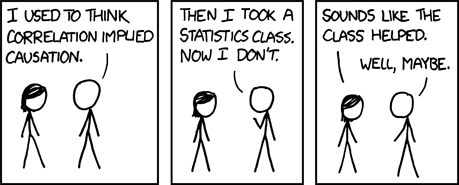
\includegraphics[width=0.5\columnwidth]{images/xkcd_correlation.png}
    \caption{A comical observation on the nature of correlation and causation. From \cite{xkcd_correlation}.}
    \label{fig:xkcd_correction}
\end{figure}


\section{Singular Value Decomposition (SVD) and Principal Component Analysis (PCA)}

We will briefly discuss the theory behind the Singular Value Decomposition and Principal Component Analysis, in order to use these as analytical techniques for correlative data later on in this thesis.

The Singular Value Decomposition, or SVD, is a way to diagonalize a given matrix in a pair of basis vectors \cite{kutz2013data}. If the matrix to be diagonalized is $A$, then the SVD may be written as
\begin{equation} \label{eq:svd}
A = \text{U} \Sigma \text{V}^{*},
\end{equation}

where \textbf{U} is a set of basis vectors expressing the range, $\Sigma$ is the diagonal matrix of singular values, and \textbf{V} is a set of basis vectors expressing the domain.

The SVD's two bases are orthonormal, and the SVD is guaranteed to exist for any matrix $A$, which cannot be said about the alternative diagonalization method of the eigenvalue decomposition \cite{kutz2013data}. The SVD allows us to project a matrix onto a new basis representation in a formal way.

Principal component analysis, or PCA, is a technique that makes heavy use of SVD. PCA takes an SVD of the covariance matrix of a series of observations in order to find the basis vectors and singular values that characterize the behavior. By looking at the magnitudes of the singular values, it becomes apparent which are significant, since the singular values are ordered and those of smaller magnitude can be elided in order to achieve a low-dimensional reduction to serve as a representation of the system \cite{kutz2013data}. This reduction consists of the ``principal components" of the system, and thus, PCA can be used to gain a fundamental understanding of how a system behaves, and how many principal modes it contains.

Note that it is important to normalize data before performing PCA, in order to avoid emphasizing data channels with large variances. Refer to \cite{shlens2014tutorial} for a detailed discussion of PCA.


\section{Visualization of Correlative Relationships}

As we discussed in the first section of this chapter, correlative relationships in a system can provide a useful view into the internal dynamics of state variables which a non-correlative approach could not. Much of the motivation behind these techniques is the discovery of new patterns and associations between variables, and as such, intuitive visualization to a human viewer is needed.

Correlative data is very high-dimensional; for a system with $n$ state variables, the correlative state looking back within a given time window is of size $\mathbb{R}^{n \times n}$. What's more, the correlative state changes over time as the time window slides across the state history, giving a total correlative state on the order of $\mathbb{R}^{n \times n \times t}$. For mission analysis over a 1,000-sample time window for an aerospace vehicle with 1,000 data channels, the correlative state has on the order of $10^{9}$ elements! Simultaneously visualizing this complex state in such a way that the data displayed to the user is maximized is a major challenge. Some of the difficulties of visualizing time series data, and the benefits of event identification and grouping, are studied in \cite{muller2003visualization}.

\subsection{Corrgrams}

A grid-based matrix representation of a matrix of correlative values, or ``corrgram," is a popular visualization used for correlation relationships in the research literature. In these visualizations, a state $\bar{x} \in \mathbb{R}^{n}$ is represented by a matrix $M \in \mathbb{R}^{n \times n}$, where $M_{ij}$ is shaded with a color hue to indicate the correlation score between $\bar{x}_{i}$ and $\bar{x}_{j}$.

\cite{yeh2007exploratory} suggests methods for visualizing correlations with schematic scatter plots and simple corrgrams. \cite{murdoch1996graphical} provides a method for more expressively visualizing correlative relationships between time series using embedded ellipse glyphs, but sacrifices dimensionality and screen space. Finally, a thorough survey of corrgram representations is given in \cite{friendly2002corrgrams}. 

For high-detail matrix structures that push the limits of on-screen display, \cite{yairi1992telemetry} shows a dense, 2D visualization of a subset of telemetry series data in which a measurement of ``association" is found through sorting, although the details of this correlative analysis are not given, and the applications were unclear to the authors at the time of the publication. Finally, \cite{cancro2007interactive} shows a colored, compact grid structure for maximizing telemetry display, although correlation is to be inferred by user inspection (i.e., noticing if two values happen to change similarly), rather than analyzed and displayed directly.

\subsubsection{Corrgram Limitations}

Corrgrams can only be used to display correlative state up to a certain level of dimensionality. After a certain point, the number of correlations which can be displayed on the screen is limited by screen space. The theoretical maximum, neglecting human perceptive limitations, would be a correlation matrix where every pixel of a screen display is used to show a different pairwise correlation. If corrgram symmetry is exploited (i.e., if we only visualize the elements above the main diagonal of the symmetric correlation matrix), we can reduce the number of visualized elements to $\frac{n^{2} - n}{2}$; however, on a generous modern screen resolution of 1920x1080, this reduces us to the capability of displaying correlations for only roughly 2,000 data channels. If we increase the pixel size to a much more reasonable 6x6 square for every data channel, we are reduced to roughly 300 displayable data channels. It is clear that screen space will be a major constraint, especially when precise interaction with the data is necessary for detailed examination.

Indeed, it does seem that interaction will be a necessity. Even with a small number of data channels, horizontal and vertical labels to show data channel identifiers will not easily fit on the screen; therefore, an interaction system for showing the channel names for data pairs of interest is necessary. This interaction load slows down usage, though, and is likely to reduce the usefulness of the visualization.

One final, major limitation of the corrgram visualization is that it only shows correlative state of the system at a single point in time; however, systems are dynamic, and their correlative states change as the systems transition between operational modes (including fault modes). If we are to see changes between modes, and to be able to identify these events as possible unmodeled faults, we need a method to see correlative data change over time.

\subsubsection{Corrgram Example}

A corrgram comparison of the Pearson Correlation Coefficient, Spearman Rank Correlation Coefficient, and Kendall Rank Correlation Coefficient is shown in Fig.~\ref{fig:correlation_comparison}. Note that the strong negative linear correlation between data channels 4 and 5 is captured well by all three correlative measurement methods; however, the strong, nonlinear association between data channels 1 and 6 is not captured as strongly by the PCC due to its inability to model nonlinear relationships.

\begin{figure}[h]
\centering
    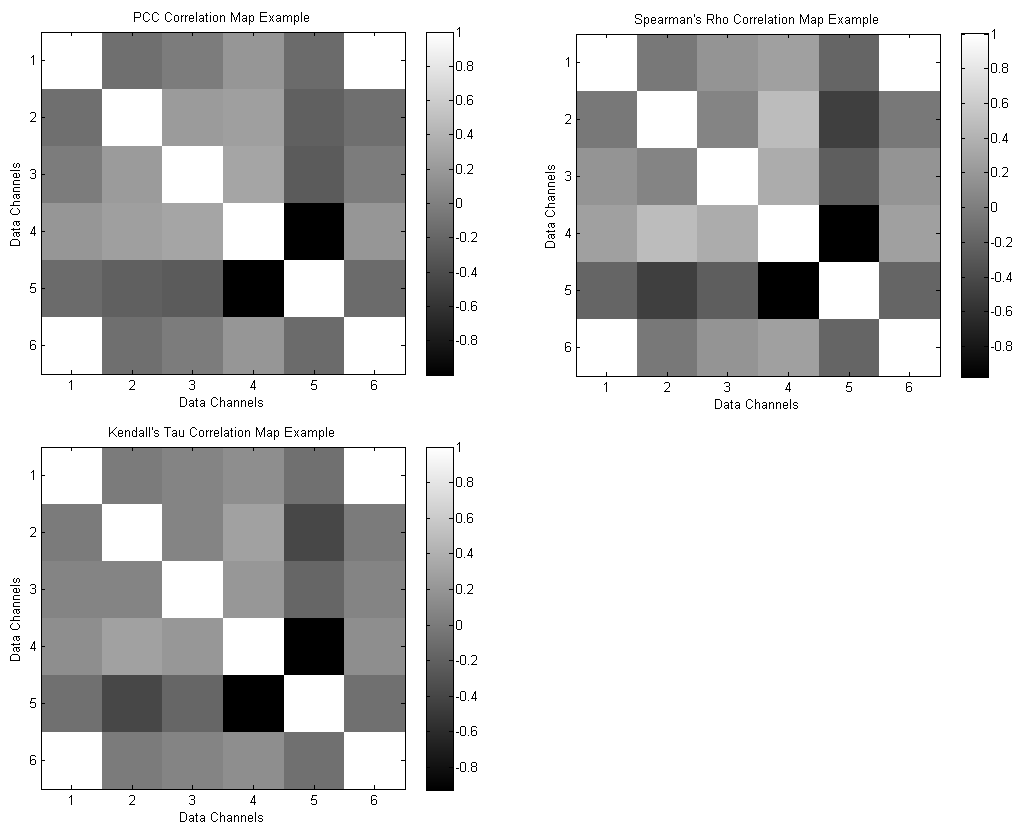
\includegraphics[width=\columnwidth]{images/correlation_comparison.png}
    \caption{Three common correlation coefficient algorithms are compared on a sample data set. Note that items 1 and 6 have a strong rank-based correlation, but the relationship is non-linear, resulting in a visibly lower correlation score within the PCC visualization. Also note the strong negative correlation between items 4 and 5.}
    \label{fig:correlation_comparison}
\end{figure}

\subsection{Animated Corrgrams}

Animated corrgrams are a potential solution to address the traditional corrgram's inability to capture changing correlative state over time. In an animated corrgram, the correlative state of a system is calculated over a retrospective time window, and every time new data is received, this correlative state is recalculated and redisplayed. This allows multiple ``views" of the current correlation during a run to be displayed, and facilitates the comparison of how correlation relationships change. We have been unable to find any examples of animated corrgrams used in previous research for displaying changing system state over time; it seems that the majority of corrgrams reviewed in the available literature operate over time-independent samples, making such a variation of limited utility.

The next chapter will walk through the creation of an animated corrgram with real system data.

% \subsection{Alternatives to Correlation Score Techniques}

% \subsection{Applications of Correlation to Residual-Based Fault Analysis}

% Though we will be primarily examining the use of correlation for data discovery and root cause diagnosis, it's worth noting that correlation state data has been successfully used in previous research to create fault detection residuals to detect an understood fault state. In \cite{isermann1984process}, Isermann 

% Isermann paper

% Discussion of how this is using correlation between telemetry values to look for an understood fault state, rather than for data discovery (but it's still valuable!)

% \subsection{Distance Correlation}

% \subsection{Correlation Ratio}

% \subsection{Brownian Covariance}

% \subsection{Coefficient of Determination}

% \subsection{Polychloric Correlation} % Correlative Analysis

\chapter{Case Study: Hakuto ``Moonraker" Lunar Rover}

In this section, we will discuss a motivating problem and platform on which to test some of the algorithms we've developed and assess their practicality.

\section{HAKUTO Lunar XPRIZE Team}

In the summer and autumn of 2015, research was performed at Tohoku University's Space Robotics Lab (hereafter ``SRL"), under the guidance of Professor Kazuya Yoshida, among others. This laboratory focuses on the research and development of robotic systems for space exploration and science missions.

One of the major sub-groups within SRL is the Hakuto Lunar XPRIZE team, a group of engineers who, in collaboration with their promotional counterparts in Tokyo, have been working for several years on the core mission of sending a lunar rover to the Moon, traveling at least 500 meters, and sending back high-resolution videos and photos. Completing this mission would satisfy the requirements of the Google Lunar XPRIZE, an international lunar rover competition with a combined purse of \$30M USD \cite{xprize}.

As a secondary mission, Hakuto hopes to explore the interior of caves on the Moon, as precursor exploration to assess their feasibility as future human habitats. Recent high-resolution photography from JAXA's Kaguya spacecraft, and from NASA's Lunar Reconnaissance Orbiter, has confirmed that large ``skylights" exist on the lunar surface leading into these caves \cite{rabbithole}, and Hakuto aims to land near enough to one of these skylights to make its exploration a possibility.

We decided that Hakuto's four-wheeled ``Moonraker" rover would be an excellent testbed against which to develop advanced fault analysis algorithms and visualizations. Moonraker is a state-of-the-art micro-rover, developed over the past 5 years by the Hakuto team \cite{walker2015update}. During normal operation, Moonraker sends back status reports on 100 to 150 channels of telemetry data to its ground station on Earth, at a rate of once per second. This telemetry covers everything from IMU attitude data and temperature sensor readings to motor rotations, solar charge voltage, and communication metadata such as packets errors and radio signal strength.

See Figure~\ref{fig:moonraker} for a photo of Moonraker.

\begin{figure}[h]
\centering
    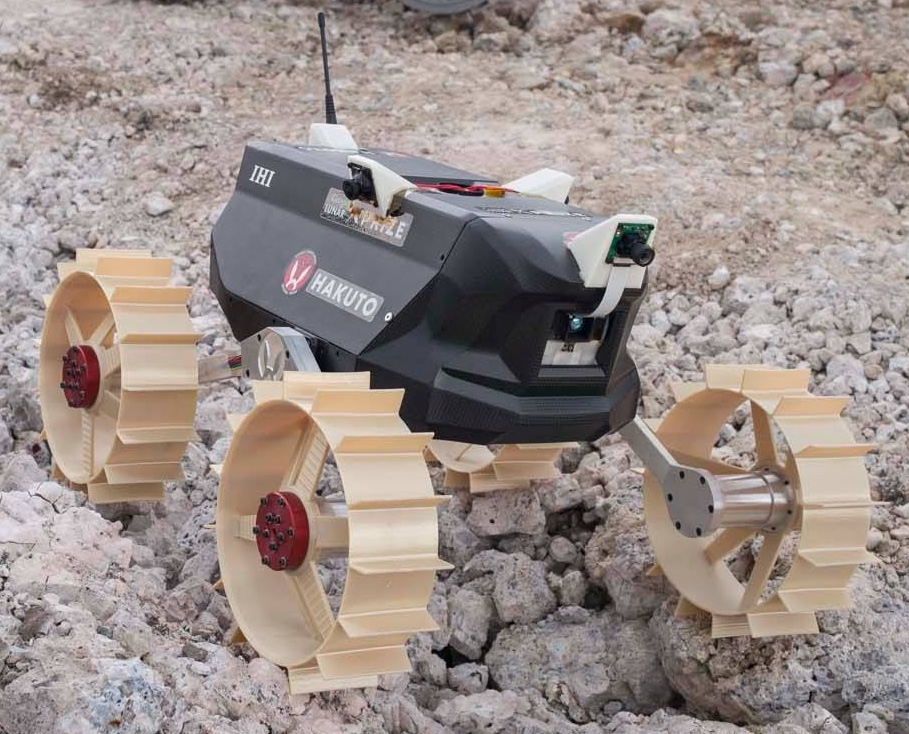
\includegraphics[width=\columnwidth]{images/moonraker.jpg}
    \caption{Hakuto's Moonraker ``Pre-Flight Model 2." Photo by George Thomas Mendel.}
    \label{fig:moonraker}
\end{figure}

\section{Ground Station Interface}

In early July 2015, Hakuto began designing a new ground station (GSN) software suite for the most recent version of the rover. Moonraker had been updated in several ways since the prior Pre-Flight Model, and many of its avionics, including its software, were updated and redesigned, breaking compatibility with the previous version of the ground station software. We worked together to evaluate the current and future needs of the rover, and to redesign and reimplement software to optimally fit these needs.

Our discussions focused on optimizing performance, reliability, and maintainability of the software. The latter factor was of particular concern, given that the software was to be used and maintained in a university laboratory environment, with many students---some of them inexperienced in software engineering---potentially responsible for updating the software and adding new features. After evaluating a list of disparate choices, including C++ on Linux with the Qt framework, and multi-platform JavaScript running in HTML5, we ultimately decided that the ideal choice would be the Unity Game Engine, for its high frequency of software updates, its active developer community, and its aerospace legacy within the NASA Jet Propulsion Laboratory \cite{jplunity}. 

\section{Rover Data Path}

In Hakuto's network configuration, Moonraker sends data packets over radio from the Moon, and they are intercepted on Earth and relayed to the ground station over the Internet. Subsequently, these packets are decoded and processed in order to be visualized by the ground station. The data is stored locally in memory by the ground station software for subsequent display. A flowchart of this data path is shown in Fig.~\ref{fig:data_path}.

\begin{figure}[h]
\centering
    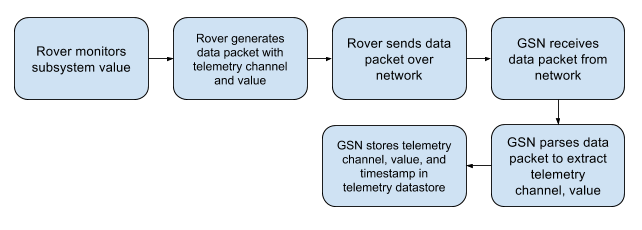
\includegraphics[width=\columnwidth]{images/rover_data_flow.png}
    \caption{Moonraker's communication flow, from rover subsystem to ground station data storage, is shown.}
    \label{fig:data_path}
\end{figure}

\subsection{Non-FDIR-Related Components}

The focus of this thesis is on the fault detective and correlative visualizations implemented within the ground station, so we will spend the bulk of the time focusing on these components. However, several non-FDIR-related components were implemented as well, briefly described below to provide context:

\begin{itemize}
    \item \textit{Numerical telemetry display}, to visually show the state of various sensors within subsystems (such as IMU accelerations, motor voltages, and board temperatures), as well as internal software metrics. Whenever possible, telemetry data was placed in semantically meaningful positions and groups, to improve discoverability.
    \item \textit{Attitude display and visual tachometer}, to provide more intuitive visualizations of pitch, roll, and current wheel rotation rate (which roughly corresponds to vehicle speed).
    \item \textit{Telemetry change indicators}, to point out data channels that have strong downward or upward trends over time.
    \item \textit{Quad-camera display}, to display the most recent images and streaming video from the rover cameras.
    \item \textit{Connectivity map}, to show the state of connectivity to various subsystems based on the elapsed time since packets from those subsystems have been received.
    \item \textit{Immersive viewing}, allowing users to view the camera data in an embedded 3D mapping.
    \item \textit{Map display}, showing the position of the rover with respect to the surrounding selenography, based on mobility subsystem and SLAM telemetry.
    \item \textit{Audio alarms}, to draw the user's attention to the UI in the event of faults.
    \item \textit{Telemetry saving, loading, and playback}, to facilitate the review of mission events after the fact.
\end{itemize}

\subsection{FDIR-Related Components}

In comparison with traditional aerospace ground station software, particular attention was given in this application to FDIR-related components. The components below were implemented and used extensively during normal operation.

\subsubsection{Threshold-based fault detection}

In order to build a threshold-based fault detection system for Moonraker, we worked with engineers on our team to define the ``danger" thresholds that indicated points of severe jeopardy, as well as the ``warning" thresholds that indicated points of concern. We implemented these thresholds in our ground station software as a general-purpose fault detection engine. Faults are detected constantly, and are displayed to the user via color and detailed information. All fault occurrence details and times are logged for future review as well. See Figure~\ref{fig:mobility_telem_subpanel}.

\begin{figure}[h]
\centering
    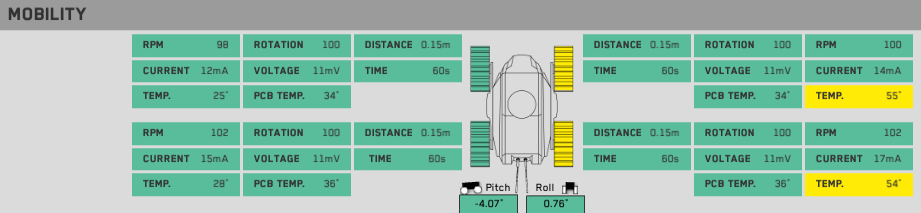
\includegraphics[width=\columnwidth]{images/mobility_telem_subpanel.png}
    \caption{Various telemetry values are shown for the mobility subsystem. Colors indicate current fault detection levels, with green representing a nominal state.}
    \label{fig:mobility_telem_subpanel}
\end{figure}

\subsubsection{Fault alert panel}

For safety, faults that have occurred need to be easily visible and understood by human operators. Towards this end, a highly visible, brightly colored alert panel was placed at the top of the screen seen by human operators. Each panel cell corresponds to a subsystem or other type of data grouping, and any issues with that grouping (i.e., faults that occur on monitored channels) will trigger a color change on that cell. Interacting with the cell can give the user more information on the fault (see the next section for details). See Figure~\ref{fig:alert_panel}.

\begin{figure}[h]
\centering
    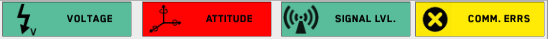
\includegraphics[width=\columnwidth]{images/alert_panel.png}
    \caption{An alert panel monitors potential faults on various different subsystems, indicating any faults and their severity by color.}
    \label{fig:alert_panel}
\end{figure}

\subsubsection{Expert fault information}

Ensuring human understanding of fault data is an essential part of the fault diagnosis and recovery process. As such, it's important to design a system where detailed information can be provided about individual faults that have occurred, while maintaining a high-level understanding of which systems are behaving anomalously. The system designed allows for this hierarchical organization of information. When high-level fault information is indicated in the ``fault alert panel," more concise information is provided in the ``fault information panel," including which anomalous data channels are contributing to the problem. The fault information is highly extensible, allowing for any other additional fault-related notes that system designers or operators would like to include for reference. This additional information, uncommon in traditional fault monitoring systems, accelerates the fault diagnosis problem by immediately pointing towards possible root causes. See Figure~\ref{fig:fault_info2}.

\begin{figure}[h]
\centering
    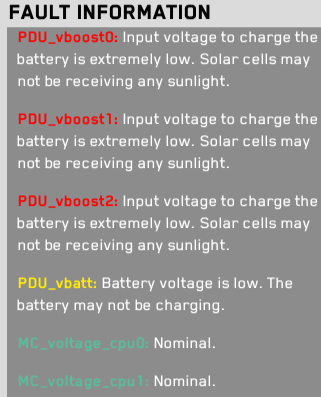
\includegraphics[width=0.4\columnwidth]{images/fault_info2.png}
    \caption{Information for monitored faults on a given subsystem.}
    \label{fig:fault_info2}
\end{figure}

\subsubsection{Correlative Functionality}

The Pearson Correlation Coefficient was chosen as an algorithm for calculating correlation between sets of data channels, in order to give a metric of their mutual ``connectedness." This algorithm was chosen for its simple and efficient calculations, under the (in retrospect, na\"{i}ve) assumption of linear relationships.

To visualize this data, a two-dimensional corrgram was used, visualizing relationships between data channels as a matrix with cell shadings representative of the PCC score of each relationship. The hue of each cell shows the sign of the correlation, and the intensity shows the strength of that correlation. This visualization allows an operator to see changing channel correlations, which may suggest possible interconnectedness or causation and aid with troubleshooting. See Figure~\ref{fig:corr_map}.

To clarify the flow of this data, pseudocode for the algorithm used is shown in Algorithm~\ref{alg:corrgram_get}. Assume that a pre-generated $n \times n$ grid of transparent blocks, $\textbf{Corr}$, is displayed on the screen. Also assume that $\textbf{GetColor}$ refers to an arbitrary function which maps from a PCC score $\in [-1,1]$ to an RGB color $(r, g, b) \in \mathbb{R}^{3}$, where $0 \leq r, g, b \leq 255$. We experimented with several variations of this function, and found that a linear mapping exaggerated the importance of low correlation scores, which led to the development of a hand-tuned exponential color mapping function to produce the correct scores. Certain work has explored the complexities of determining a proper mapping, which relate to the non-linearity of human perception of color \cite{friendly2002corrgrams}. Other work has suggested the efficacy of pre-squaring the PCC score before display, which instead results in displaying the coefficient of determination (i.e., the shared portion of the variance) for the pair of data items, which incidentally corresponds to a more intuitive human understanding of data connectivity \cite{rummelcorrelation}.

\begin{algorithm}
    \caption{Animated Corrgram Generation Algorithm}\label{alg:corrgram_get}
    \begin{algorithmic}[1]
        \Procedure{CorrgramGenerator}{$M$}\Comment{Takes data matrix $M \in \mathbb{R}^{n \times t}$.}
        \State $M_{r} \gets \{U_{:,j}\}_{j=t-s}^{n}$ \Comment{Reduce data to most recent $s$ points.}
        \State $C\gets \textbf{PCC}_{s}(M_{r})$ \Comment{Calculate a symmetric PCC matrix using last $s$ points.}
        \For{$\textbf{row} = 1~\textbf{to}~n$}
            \For{$\textbf{col} = 1~\textbf{to}~n$}
                \State $\textbf{color} = \textbf{GetColor}(C_{row, col})$ \Comment{Convert PCC score to a color.}
                \State $\textbf{Corr}_{row, col}\textbf{.color} \gets \textbf{color}$ \Comment{Assign color to cell in corrgram.}
            \EndFor
        \EndFor
        \EndProcedure \Comment{Algorithm is re-run on every graphical update.}
    \end{algorithmic}
\end{algorithm}

A few additional modifications were applied in order to make this algorithm performant. For instance, the entire corrgram is not updated at once, due to the performance hit from calculating new PCC scores for thousands of corrgram cells on each graphical update. Instead, a subset of the corrgram cells are updated, resulting in a ``rolling" effect wherein cells update gradually, with a full update of the corrgram being achieved on the order of once per second.

We also built functionality to adjust the sampling rate, the period of time over which samples are taken, and parameters related to averaging for smoothing out noise. Channel pairs may also be filtered via substring search, or via current fault states.

\begin{figure}[h]
\centering
    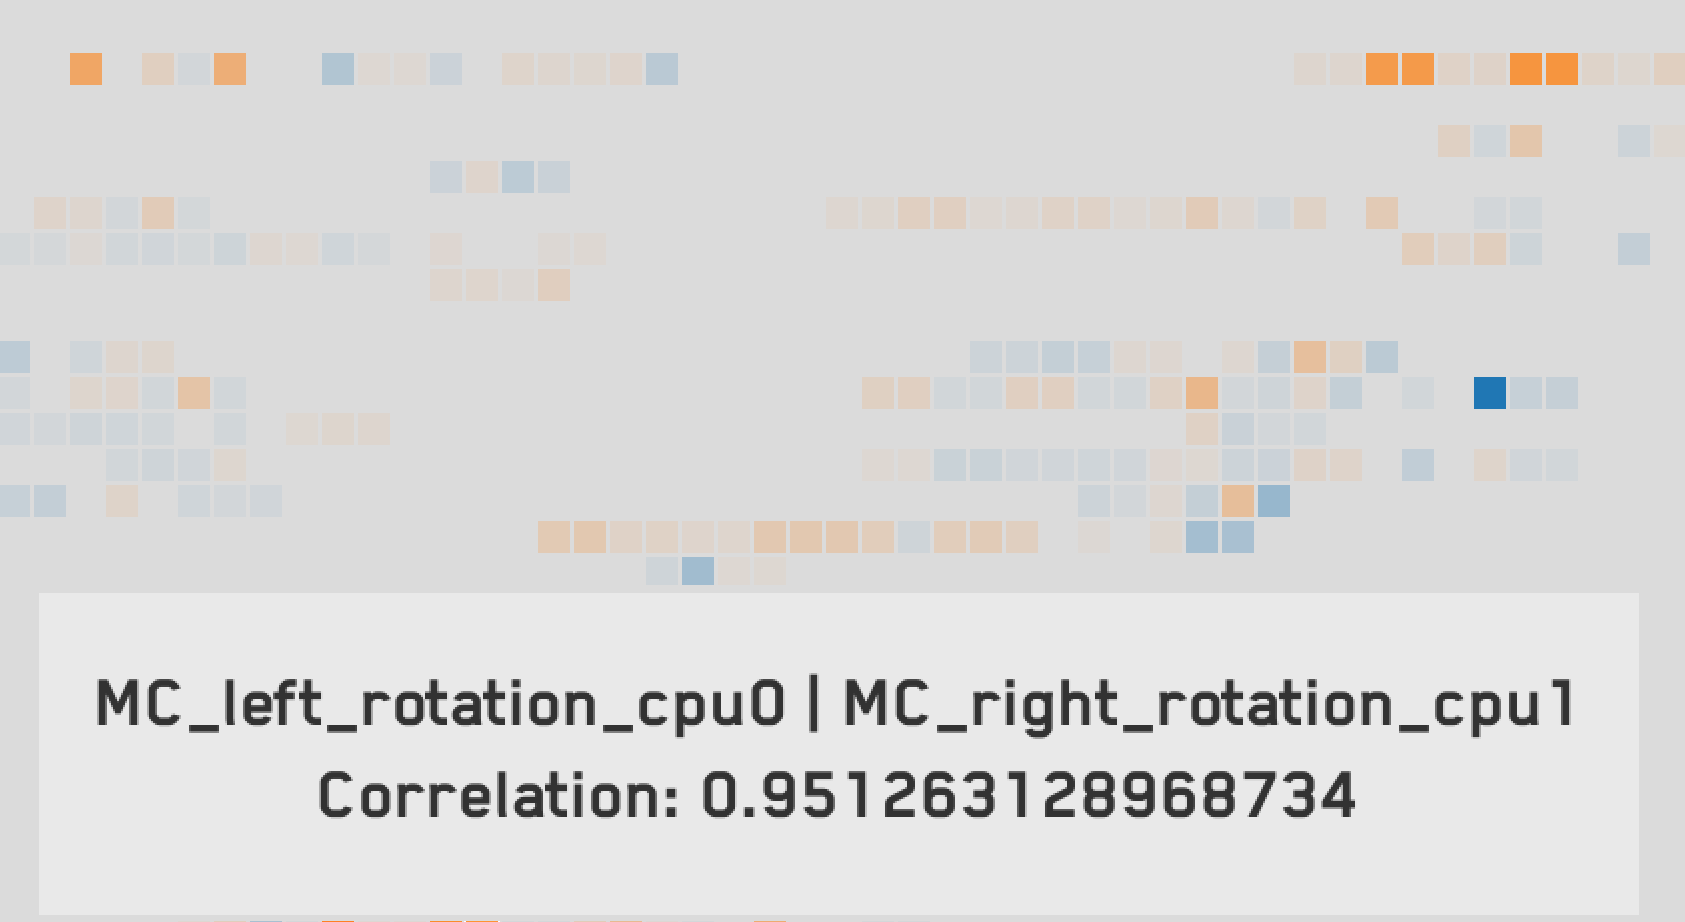
\includegraphics[width=\columnwidth]{images/corr_map.png}
    \caption{Correlation map visualization showing various different data channel pairs and their correlations. Bright orange signifies a high positive correlation, and bright blue is a high negative correlation.}
    \label{fig:corr_map}
\end{figure}

The next chapter will discuss testing we performed to validate the various components of this ground station interface. % Visualization of Correlative Relationships

\chapter{Case Study: Hakuto ``Moonraker" Lunar Rover}

In this section, we will discuss a motivating problem and platform on which to test some of the algorithms we've developed and assess their practicality.

\section{HAKUTO Lunar XPRIZE Team}

In the summer and autumn of 2015, research was performed at Tohoku University's Space Robotics Lab (hereafter ``SRL"), under the guidance of Professor Kazuya Yoshida, among others. This laboratory focuses on the research and development of robotic systems for space exploration and science missions.

One of the major sub-groups within SRL is the Hakuto Lunar XPRIZE team, a group of engineers who, working together with their promotional counterparts in Tokyo, have been working for several years on the core mission of sending a lunar rover to the Moon, traveling at least 500 meters, and sending back high-resolution and photos. Completing this mission would satisfy the requirements of the Google Lunar XPRIZE, an international lunar rover competition with a combined purse of \$30M USD \cite{xprize}.

As a secondary mission, Hakuto hopes to explore the interior of caves on the Moon, as precursor exploration to assess their feasibility as future human habitats. Recent high-resolution photography from JAXA's Kaguya spacecraft, and from NASA's Lunar Reconnaissance Orbiter, has confirmed that large ``skylights" exist on the lunar surface leading into these caves \cite{rabbithole}, and Hakuto aims to land near enough to one of these skylights to make its exploration a possibility.

We decided that Hakuto's four-wheeled ``Moonraker" rover would be an excellent testbed against which to develop advanced fault analysis algorithms and visualization. Moonraker is a state-of-the-art micro-rover, developed over the past 5 years by the Hakuto team. During normal operation, Moonraker sends back status reports on 100 to 150 channels of telemetry data to its ground station on Earth, at a rate of once per second. This telemetry covers everything from IMU attitude data and temperature sensors readings to motor rotations, solar charge voltage, and communication metadata such as packets errors detected and radio signal strength.

See Figure~\ref{fig:moonraker} for a photo of Moonraker.

\begin{figure}[h]
\centering
    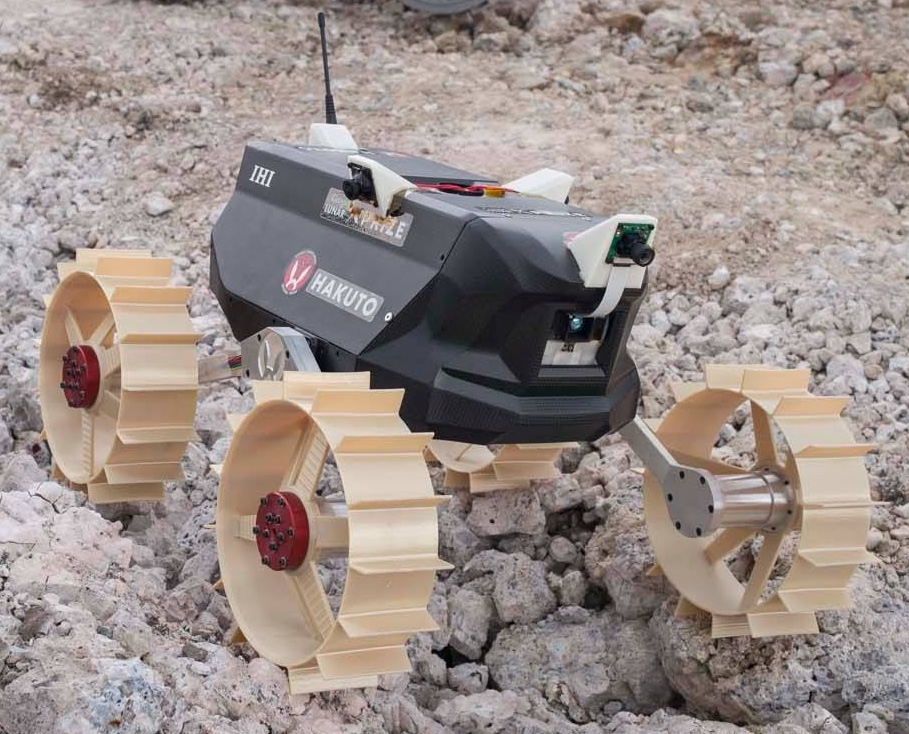
\includegraphics[width=\columnwidth]{images/moonraker.jpg}
    \caption{Hakuto's Moonraker ``Pre-Flight Model 2." Photo by George Thomas Mendel.}
    \label{fig:moonraker}
\end{figure}

\section{Ground Station Interface}

In early July 2015, Team Hakuto began designing a new ground station software suite for the most recent version of the rover. The rover had been updated in several ways since the prior Pre-Flight Model, and many of its avionics, including its software, were updated and redesigned, breaking compatibility with the previous version of the ground station software. We worked together to evaluate the current and future needs of the rover, and to redesign and reimplement software to optimally fit these needs.

Our discussions focused on optimizing performance, reliability, and maintainability of the software. The latter factor was of particular concern, given that the software was to be used and maintained in a university laboratory environment, with many students---some of them inexperienced in software engineering---potentially responsible for updating the software and adding new features. After evaluating a list of disparate choices, including C++ on Linux with the Qt framework and multi-platform JavaScript running in HTML5, we ultimately decided that the ideal choice would be the Unity Game Engine, for its high frequency of software updates, its active developer community, and its aerospace legacy within the NASA Jet Propulsion Laboratory \cite{jplunity}. 

\section{Rover Data Path}

In Hakuto's network configuration, Moonraker sends data packets over radio from the Moon, and they are intercepted on Earth and relayed to the ground station over the Internet. Subsequently, these packets are decoded and processed in order to be visualized by the ground station. The data is stored locally in memory by the ground station software for subsequent display. A flowchart of this data path is shown in Fig.~\ref{fig:data_path}.

\begin{figure}[h]
\centering
    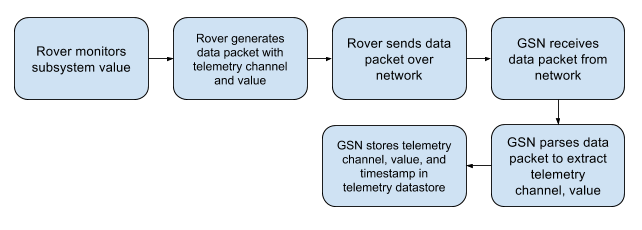
\includegraphics[width=\columnwidth]{images/rover_data_flow.png}
    \caption{Moonraker's communication flow, from rover subsystem to ground station data storage, is shown.}
    \label{fig:data_path}
\end{figure}

\subsection{Non-FDIR-Related Components}

The focus of this paper is on the fault detective and correlative visualizations implemented within the ground station, so we will spend the bulk of the time focusing on this component. However, there were several non-FDIR-related components as well, briefly described below to provide context:

\begin{itemize}
    \item \textit{Numerical telemetry display}, to visually show the state of various sensors on subsystem boards (such as IMU accelerations, motor voltages, and board temperatures), as well as internal software metrics. Whenever possible, telemetry data was placed in semantically meaningful positions and groups, to improve discoverability.
    \item \textit{Attitude display and visual tachometer}, to provide more intuitive visualizations of pitch, roll, and current wheel rotation rate (which mostly corresponded to vehicle speed).
    \item \textit{Telemetry change indicators}, to point out data channels that have strong downward or upward trends over time.
    \item \textit{Quad-camera display}, to display the most recent images and streaming video from the rover cameras.
    \item \textit{Connectivity map}, to show the state of connectivity to various subsystems based on the elapsed time since packets from those subsystems had been received.
    \item \textit{Immersive viewing}, allowing users to navigate the camera data in an embedded 3D mapping.
    \item \textit{Map display}, showing the position of the rover with respect to the surrounding selenography, based on mobility subsystem telemetry and SLAM telemetry.
    \item \textit{Audio alert cues}, to draw the user's attention to the UI in the event of faults.
    \item \textit{Telemetry saving, loading, and playback}, to facilitate the review of mission events after the fact.
\end{itemize}

\subsection{FDIR-Related Components}

In comparison with traditional aerospace ground station software, particular attention was given in this implementation to FDIR-related components. The components below were implemented and used extensively.

\subsubsection{Threshold-based fault detection}

In order to build a threshold-based fault detection system for Moonraker, we worked with engineers on our team to define the ``danger" thresholds that indicated points of severe jeopardy, as well as the ``warning" thresholds that indicated points of concern. We implemented these thresholds in my ground station software as a general-purpose fault detection engine. Faults are detected constantly, and are displayed to the user via color and detailed information (see the following sections for more details). All fault occurrence details and times are logged for future review as well. See Figure~\ref{fig:mobility_telem_subpanel}.

\begin{figure}[h]
\centering
    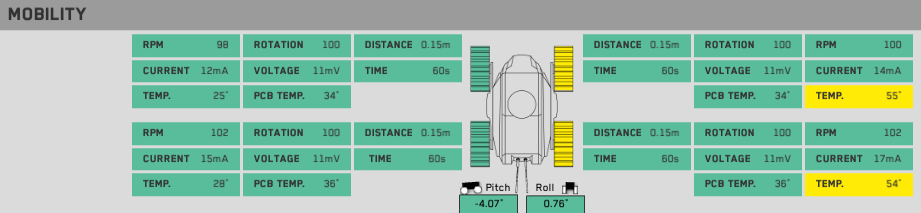
\includegraphics[width=\columnwidth]{images/mobility_telem_subpanel.png}
    \caption{Various telemetry values are shown for the mobility subsystem. Colors indicate current fault detection levels, with green representing a nominal state.}
    \label{fig:mobility_telem_subpanel}
\end{figure}

\subsubsection{Fault alert panel}

For safety, faults that have occurred need to be easily visible and understood by human operators. Towards this end, a highly visible, brightly colored alert panel was placed at the top of the screen seen by human operators. Each panel cell corresponds to a subsystem or other type of data grouping, and any issues with that grouping (i.e., faults that occur on monitored channels) will trigger a color change on that cell. Interacting with the cell can give the user more information on the fault (see the next section for details). See Figure~\ref{fig:alert_panel}.

\begin{figure}[h]
\centering
    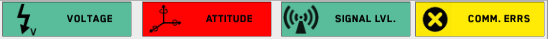
\includegraphics[width=\columnwidth]{images/alert_panel.png}
    \caption{An alert panel monitors potential faults on various different subsystems, indicating any faults and their severity by color.}
    \label{fig:alert_panel}
\end{figure}

\subsubsection{Expert fault information}

Ensuring human understanding of fault data is an essential part of the fault diagnosis and recovery process. As such, it's important to design a system where detailed information can be provided about individual faults that have occurred, while maintaining a high-level understanding of which systems are behaving anomalously. The system designed allows for this hierarchical organization of information. When high-level fault information is indicated in the ``fault alert panel," more concise information is provided in the ``fault information panel," including which anomalous data channels are contributing to the problem. The fault information is highly extensible, allowing for any other additional fault-related notes that system designers or operators would like to include for reference. This additional information, uncommon in traditional fault monitoring systems, accelerates the fault diagnosis problem by immediately pointing towards possible root causes. See Figure~\ref{fig:fault_info2}.

\begin{figure}[h]
\centering
    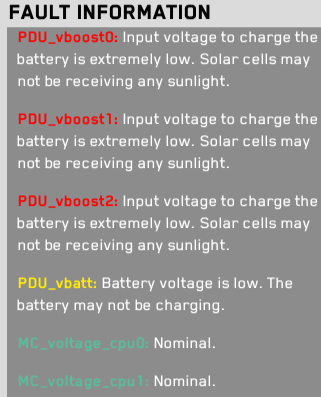
\includegraphics[width=0.4\columnwidth]{images/fault_info2.png}
    \caption{Information for monitored faults on a given subsystem.}
    \label{fig:fault_info2}
\end{figure}

\subsubsection{Correlative Functionality}

The Pearson Correlation Coefficient was chosen as an algorithm for calculating correlationbetween sets of data channels, in order to give a metric of their mutual ``connectedness." This algorithm was chosen for its simple and efficient calculations, under the (in retrospect, naïve) assumption of linear relationships.

To visualize this data, a two-dimensional corrgram was used, visualizing relationships between data channels as a matrix with cell shadings representative of the PCC score of each relationship. Hue of each cell shows positive/negative correlation, and intensity shows the strength of that correlation. This visualization allows an operator can see changing channel correlations, which may suggest possible interconnectedness or causation and aid with troubleshooting. See Figure~\ref{fig:corr_map}.

To show the flow of this data, pseudocode for the algorithm used is shown in Algorithm~\ref{alg:corrgram_get}. Assume that a pre-generated $n \times n$ grid of transparent blocks, $\textbf{Corr}$, is displayed on the screen. Also assume that $\textbf{GetColor}$ refers to an arbitrary function which maps from a PCC score $\in [-1,1]$ to an RGB color $(r, g, b) \in \mathbb{R}^{3}$, where $0 \leq r, g, b \leq 255$. We experimented with several variations of this function, and found that a linear mapping exaggerated the importance of low correlation scores, which led to the development of a hand-tuned exponential color mapping function to produce the correct scores. Certain work has explored the complexities of determining a proper mapping, which relate to the non-linearity of human perception of color \cite{friendly2002corrgrams}. Other work has suggested the efficacy of pre-squaring the PCC score before display, which instead results in displaying the coefficient of determination (i.e., the shared portion of the variance) for the pair of data items, which intuitively corresponds to a more intuitive human understanding of data connectivity \cite{rummelcorrelation}.

\begin{algorithm}
    \caption{Animated Corrgram Generation Algorithm}\label{alg:corrgram_get}
    \begin{algorithmic}[1]
        \Procedure{CorrgramGenerator}{$D$}\Comment{Takes data point matrix $D \in \mathbb{R}^{n \times t}$.}
        \State $S \gets \{U_{:,j}\}_{j=t-s}^{n}$ \Comment{Reduce data to most recent $s$ points.}
        \State $P\gets \textbf{PCC}_{s}(D_{r})$ \Comment{Calculate a symmetric PCC matrix using last $s$ points.}
        \For{$\textbf{row} = 1~\textbf{to}~n$}
            \For{$\textbf{col} = 1~\textbf{to}~n$}
                \State $\textbf{color} = \textbf{GetColor}(S_{row, col})$ \Comment{Convert PCC score to a color.}
                \State $\textbf{Corr}_{row, col}\textbf{.color} \gets \textbf{color}$ \Comment{Assign color to cell in corrgram.}
            \EndFor
        \EndFor
        \EndProcedure \Comment{Algorithm is re-run on every graphical update.}
    \end{algorithmic}
\end{algorithm}

A few additional modifications were applied in order to make this algorithm performant. For instance, the entire corrgram is not updated at once, due to the performance hit from calculating new PCC scores for thousands of corrgram cells on each graphical update. Instead, a subset of the corrgram cells are updated, resulting in a ``rolling" effect wherein cells update gradually, with a full update of the corrgram being achieved on the order of once per second.

We also built functionality to adjust the sampling rate, the period of time over which samples are taken, and parameters related to averaging for smoothing out noise. Channel pairs may also be filtered via substring search.

\begin{figure}[h]
\centering
    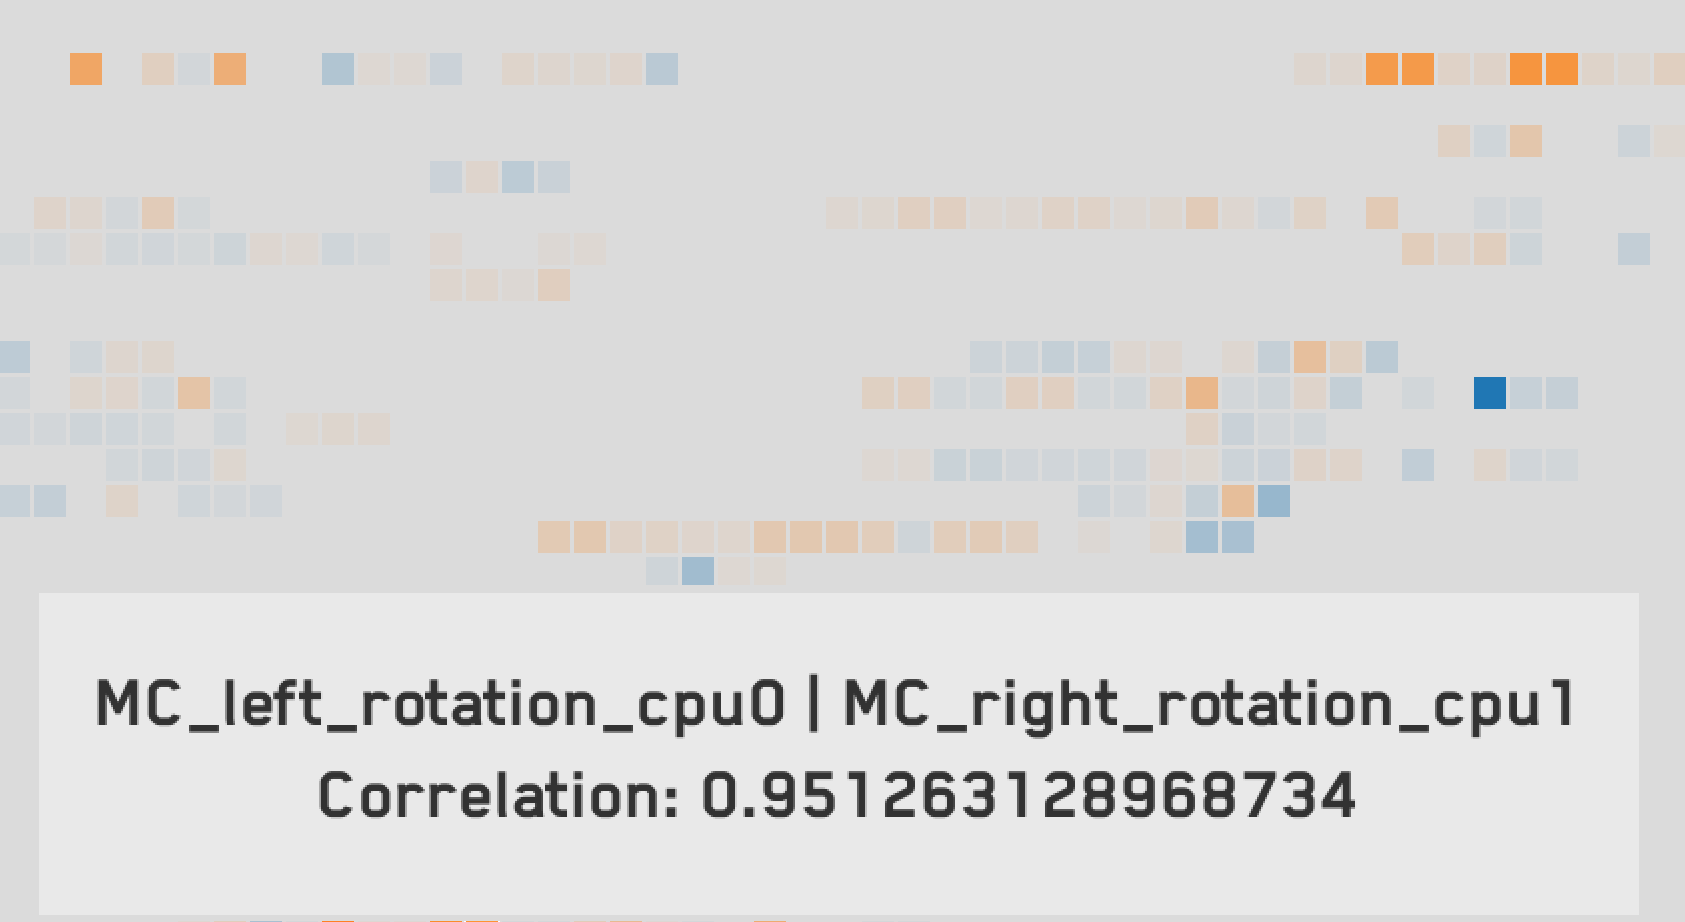
\includegraphics[width=\columnwidth]{images/corr_map.png}
    \caption{Correlation map visualization showing various different data channel pairs and their correlations. Bright orange signifies a high positive correlation, and bright blue is a high negative correlation.}
    \label{fig:corr_map}
\end{figure}

\section{Testing}

Hakuto carried out a number of field tests on the ground station software, including FDIR-related and correlative components. The major tests we conducted are described in detail below.

\subsection{Field Testing}

Over the course of two weeks, we performed daily field tests in the rock quarry, to both assess the physical characteristics of our radio communication and to confirm our mobility in a simulated lunar environment. (See Fig.~\ref{fig:night_test_team} for an image of the quarry terrain.) The ground station interface was in constant use throughout the course of the tests, with alternating drivers at the helm. The setup usually involved one primary pilot and one copilot, who helped with troubleshooting. See Fig.~\ref{fig:daytime_operation_pittsburgh_field_test} for an image of normal operation.

Our radio testing was multi-pronged. First, we endeavored to established that we could a) communicate from the ground station to Moonraker and vice-versa by going through Astrobotic's radio relay, which they set up to emulate their lunar lander which will function as a communication relay during the actual, planned lunar mission. Second, we tested the communication capabilities of Moonraker's radio antenna at two different operating frequencies (900 MHz and 2.4 GHz), in order to characterize performance over long distance and with line-of-sight blocked by rocky terrain. We looked for communication signal strength and commanding efficacy in the presence of packet loss, and also tested the effect of a signal strength amplifier in a poor connectivity situation. These results were promising and are currently being analyzed by our communications team.

Our mobility testing consisted of driving long distances over rocky, yet generally even, terrain, occasionally using only the near-real-time (``NRT") streaming video telemetry as visual feedback. We set up various challenges, such as large rock obstacles and inclines of increasing steepness, to test the rover's mobility capabilities as well as our operational capabilities using the ground station interface.

Other tasks performed during the field tests included coordinating with Hakuto crew and Astrobotic/Caltech engineers to fulfill mission tasks, scouting for field test locations, setting up and testing the ground station and radio equipment, and driving the rover during all of the tests to accomplish all of our test goals.

Results of this field test, and other similar ones, will be discussed in the next chapter.

\begin{figure}[h]
\centering
    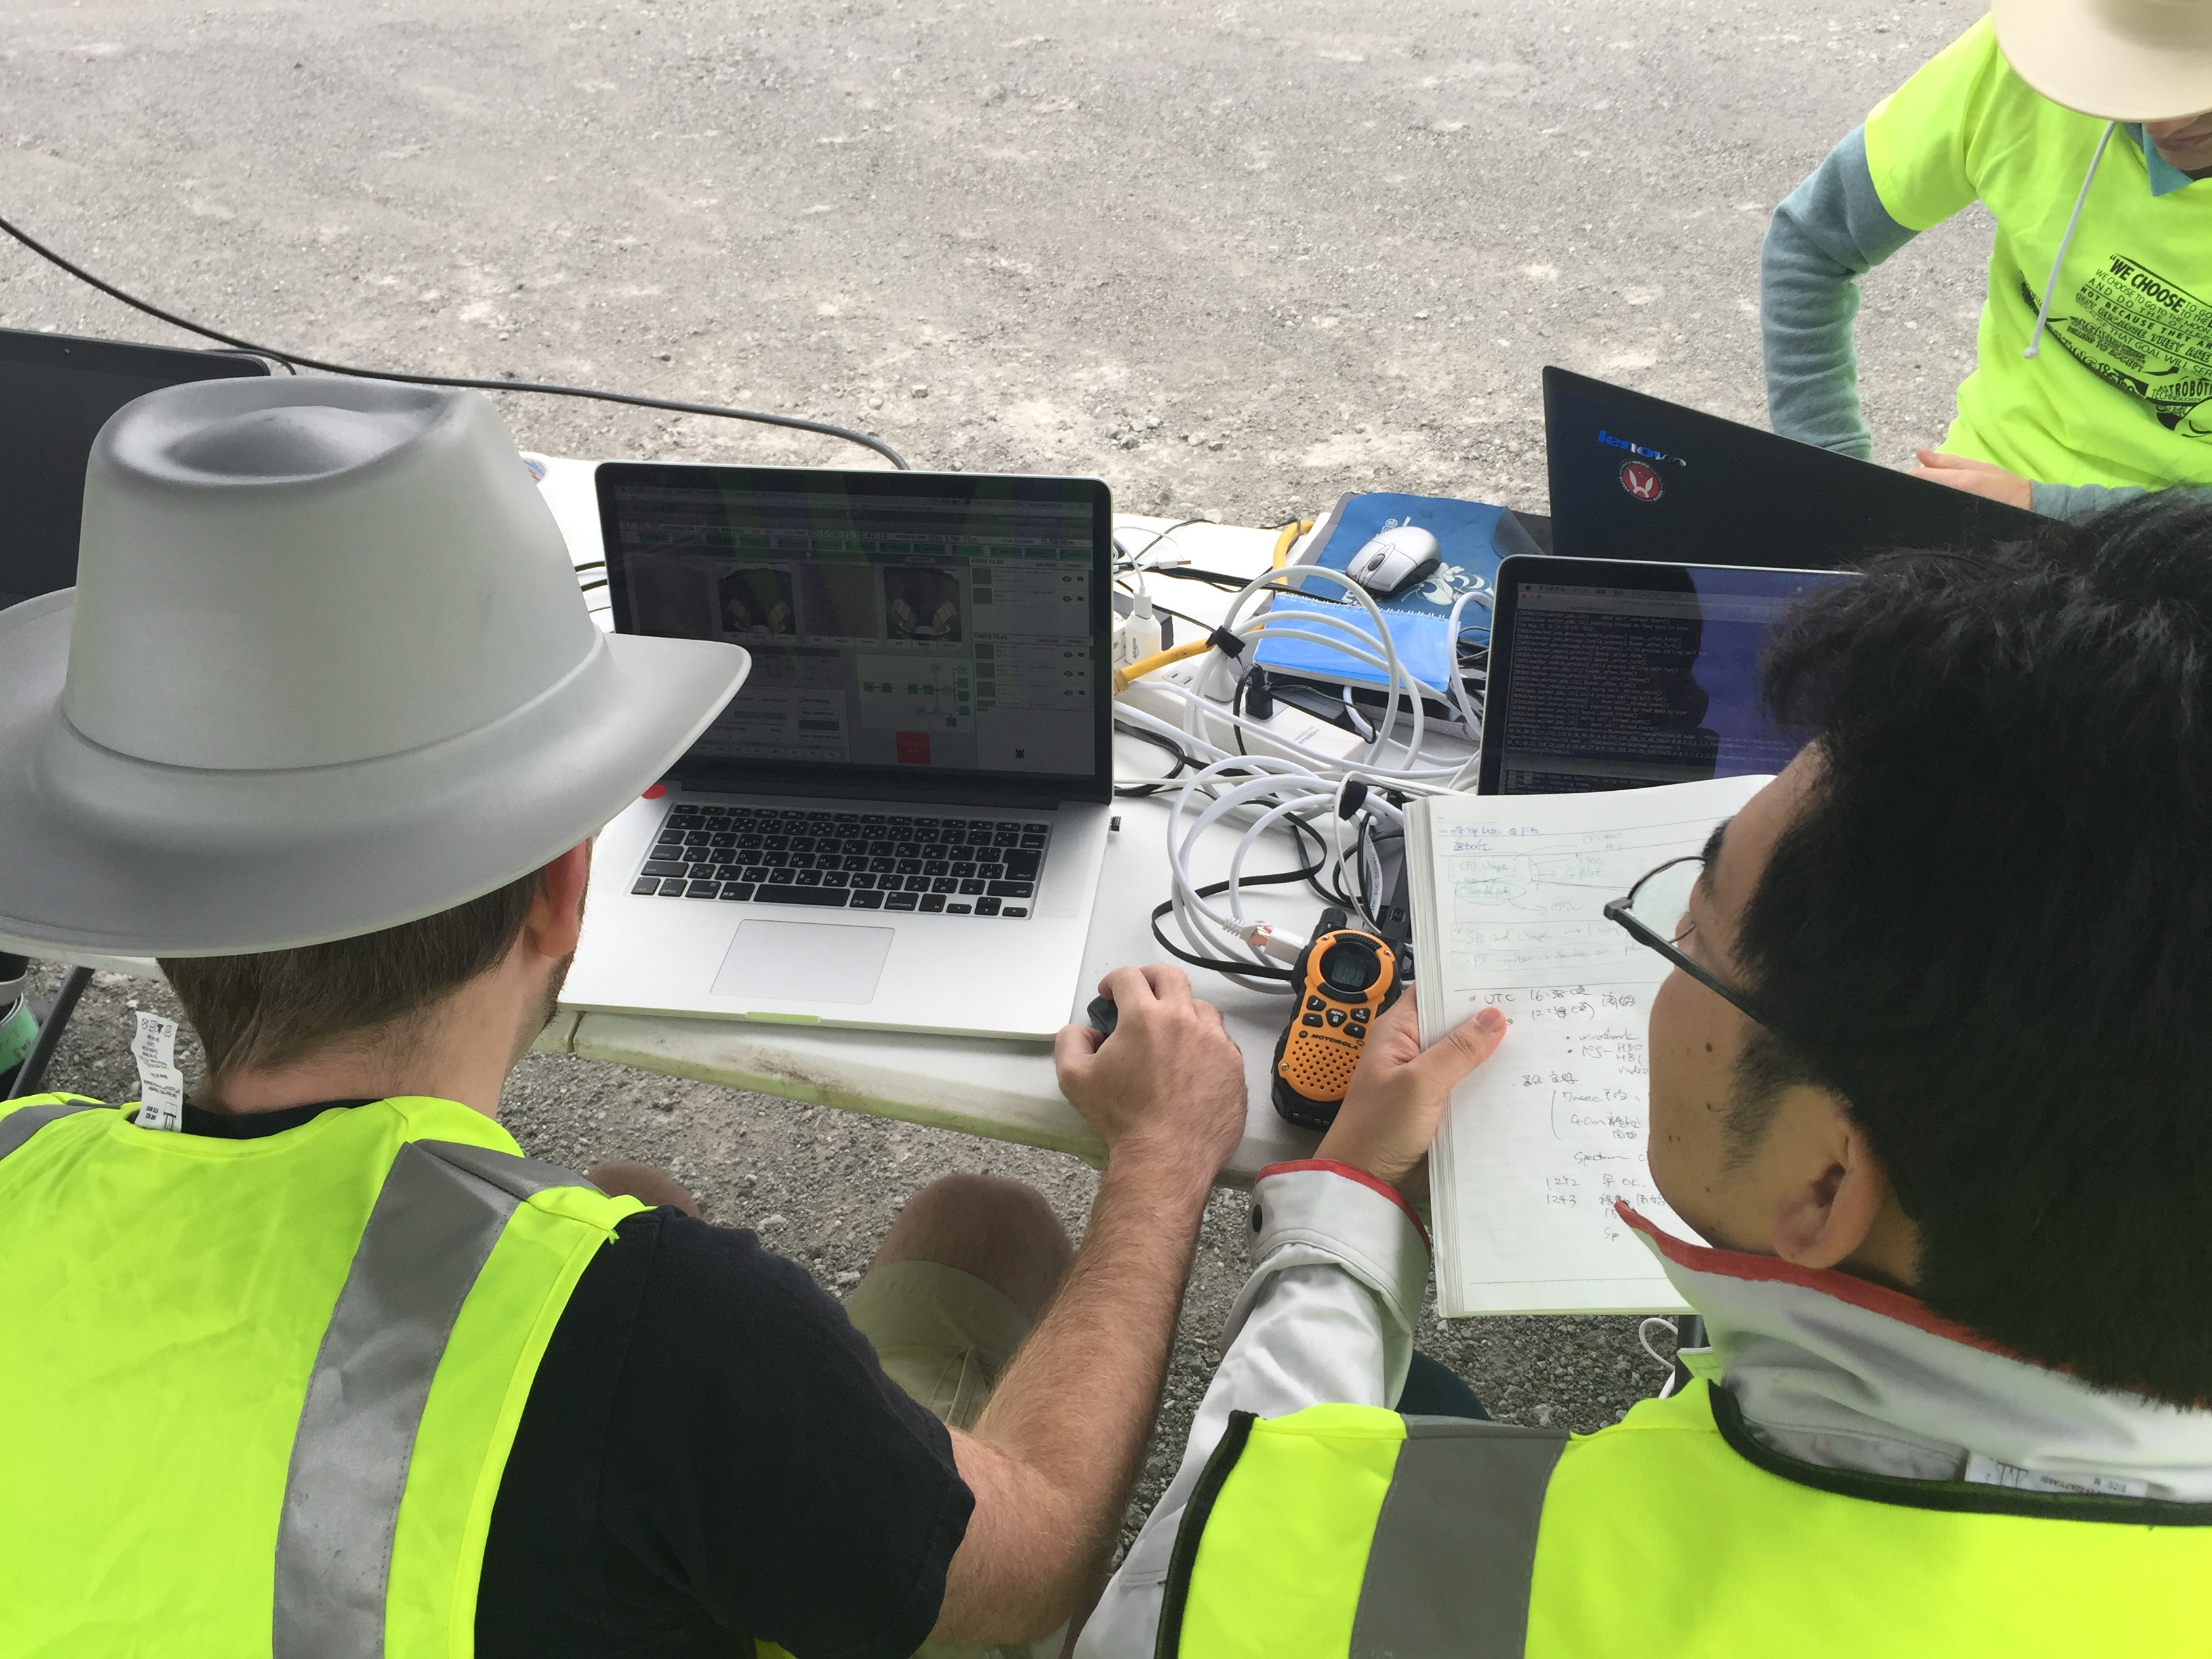
\includegraphics[width=\columnwidth]{images/daytime_operation_pittsburgh_field_test.jpg}
    \caption{Lead software engineer Toshiro Shimizu and the author work on radio testing during a Pittsburgh field test at the Lafarge rock quarry.}
    \label{fig:daytime_operation_pittsburgh_field_test}
\end{figure}

\begin{figure}[h]
\centering
    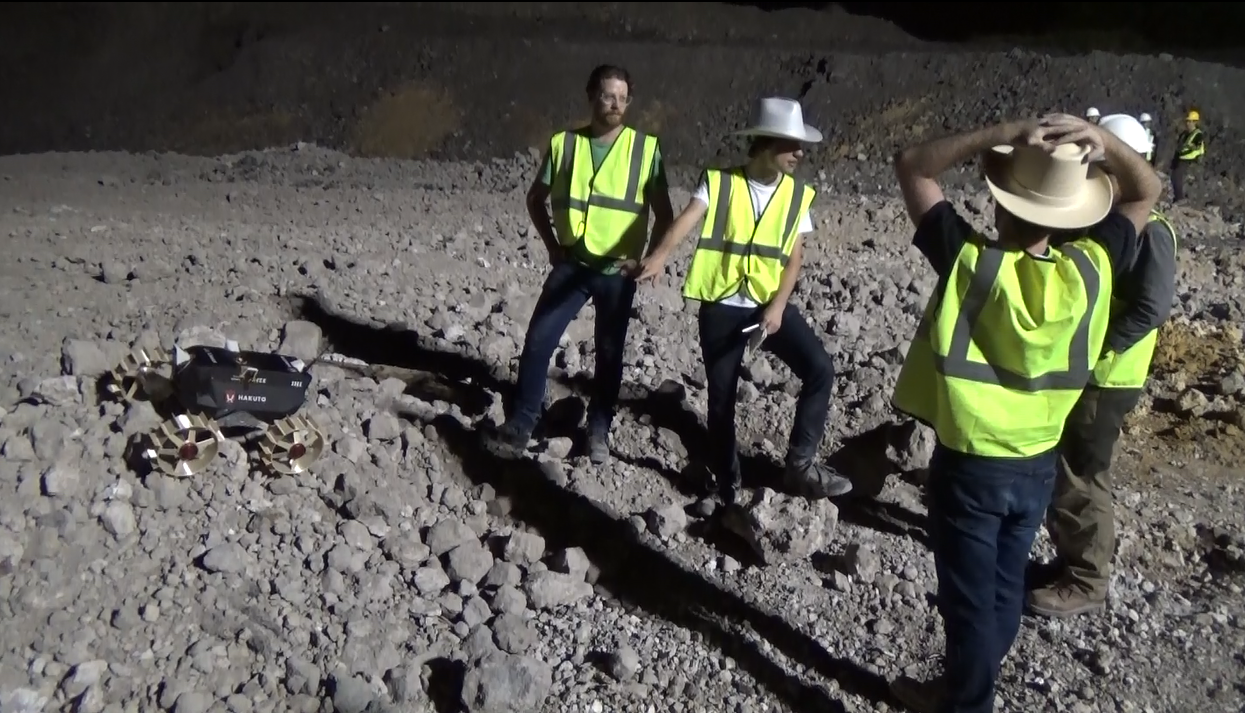
\includegraphics[width=\columnwidth]{images/night_test_team.png}
    \caption{Engineering members of Team Hakuto discuss terrain challenges during a nighttime field test.}
    \label{fig:night_test_team}
\end{figure}

\subsection{Usability Testing}

In November 2015, we performed a set of usability tests on a slimmed-down version of the Moonraker ground station interface, in order to evaluate the various data analysis affordances and to determine any usability issues in need of attention. Seven users participated in the test, mostly interns and students possessing some familiarity with the rover, but with limited to no experience operating it via the ground station interface. See Fig.~\ref{fig:ui_test_takako} for an image of a user taking the test.

\begin{figure}[h]
\centering
    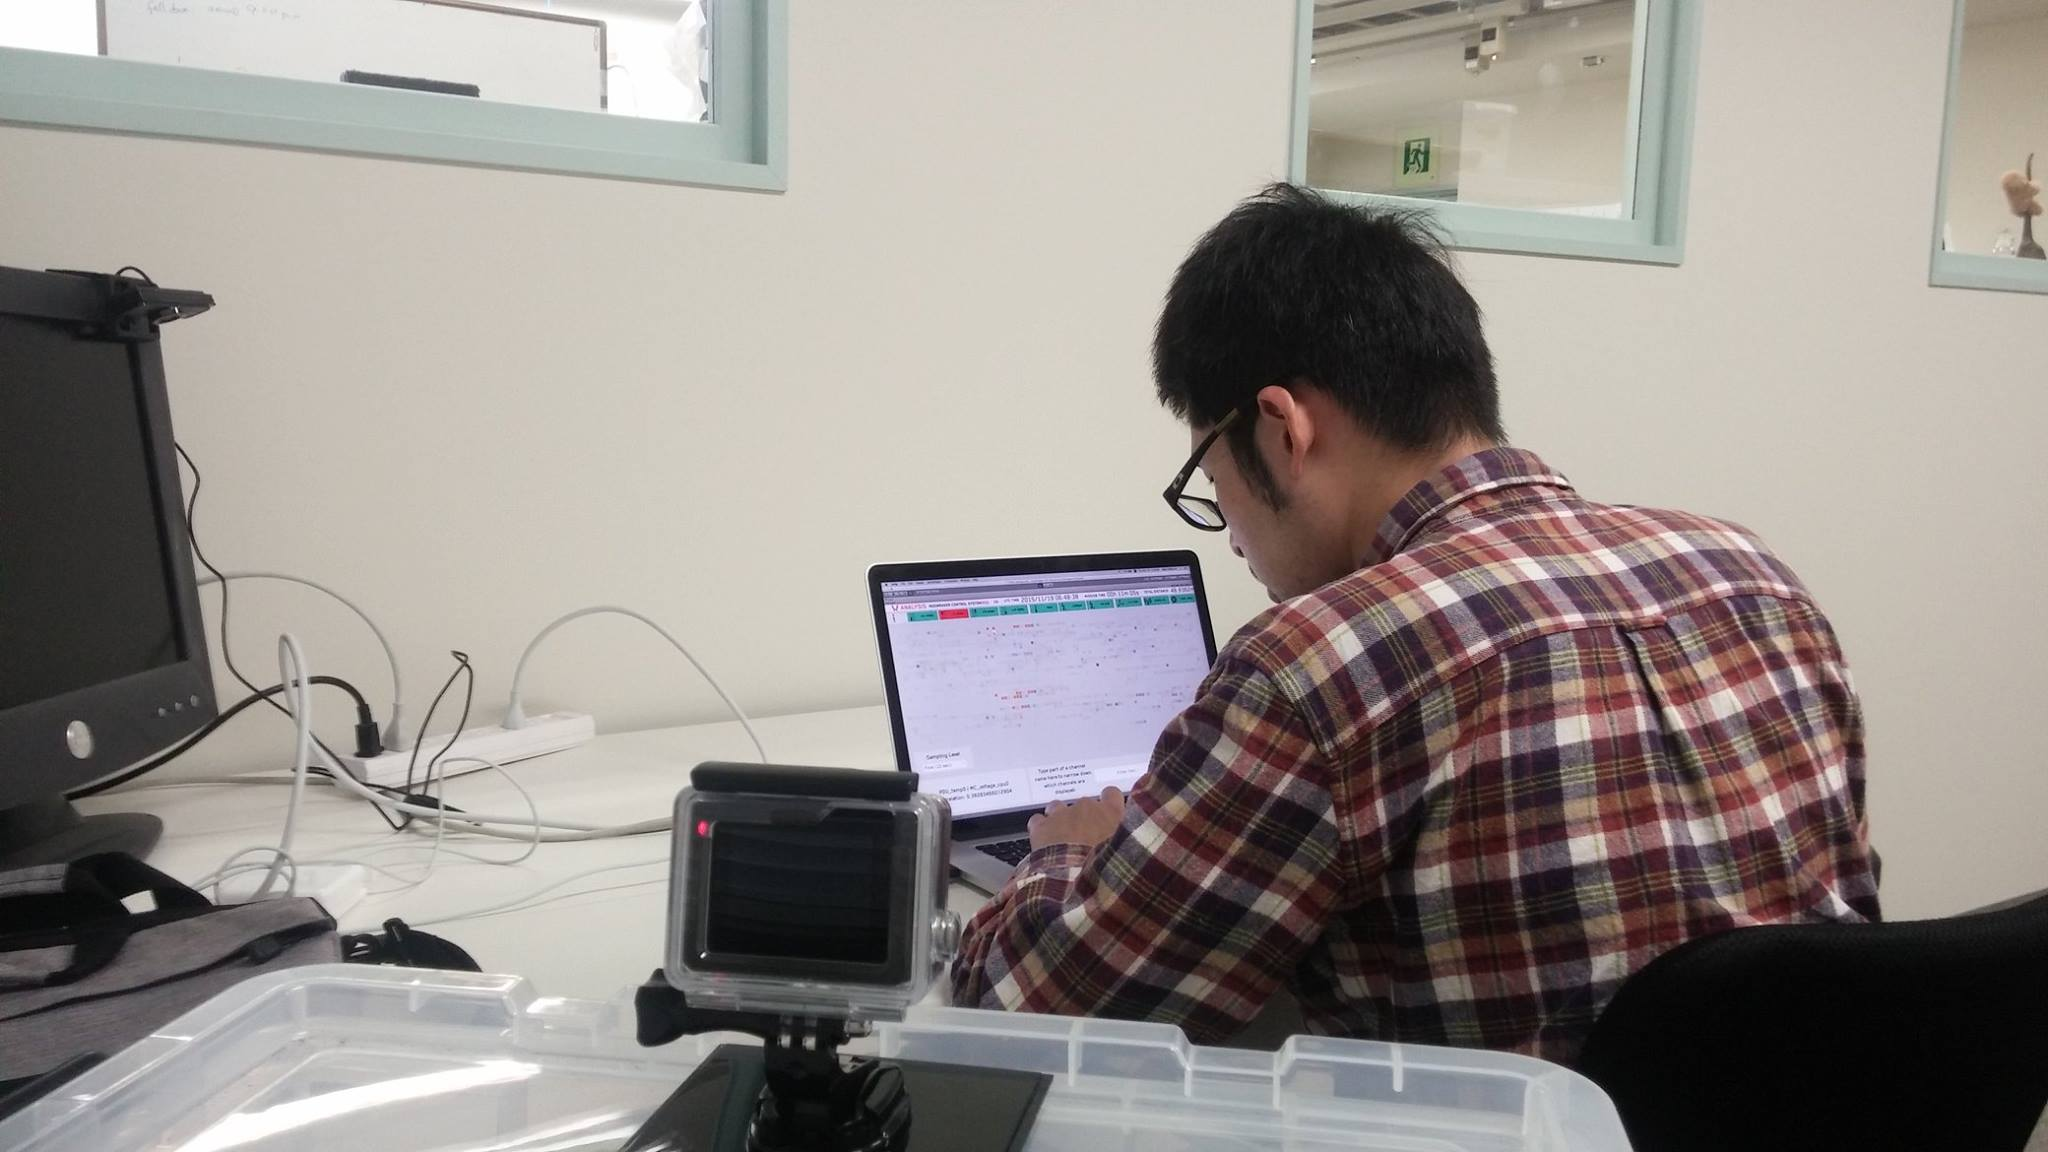
\includegraphics[width=\columnwidth]{images/ui_test_takuto.jpg}
    \caption{A usability test participant focuses on the incoming telemetry to try to ascertain patterns behind a faulted system.}
    \label{fig:ui_test_takako}
\end{figure}

Participants were presented with a simplified form of the ground station, with the Pilot Screen, Copilot Screen, and the Correlation Map screen. As the correlation map is a relatively novel idea, and has not (to the best of the author's knowledge) ever been used in ground station software, this test also served to see if it could be immediately usable in its present state, or if special training or modifications will be necessary before the correlation map is useful for correlation discovery and root cause analysis.

\subsubsection{Test Tasks}

During the test, participants monitored telemetry and looked for patterns in received data during a ~10-minute simulation drive on the lunar surface. During the course of the drive, camera images were unavailable, but the rover telemetry was indicative of various events that occurred to the rover during the run. The scenario consisted of the rover descending down into a crater, where it loses direct sunlight, resulting in reduced temperatures and solar charge voltages. It also loses line of sight with the lunar lander, causing packet losses and a reduction in signal strength. The rover then climbs out of the crater, bringing about an all-around improvement in these conditions. It enters some rough terrain, and ultimately stops after a rock becomes stuck in the wheel.

It was the task of the usability test participants to analyze the telemetry as it was received in order to try to understand the details of the story above. After the 10-minute run was complete, users were then given up to an additional 10 minutes to review received telemetry until they were satisfied they had understood the ``story" of the rover's trip.

Results of usability testing will be discussed in the next chapter. % Case Study: Hakuto ``Moonraker" Lunar Rover

\chapter{Intermediate Results and Reassessment}

This chapter discusses some of the learnings from our intermediate testing, and how we used them to shape our next steps for correlative assessment techniques.

\section{Field Test Results}

Our field tests went swimmingly, and we returned to Japan with excellent results and ideas for improvement, but these tests were not without a small number of issues. We uncovered several minor bugs within the ground station, which were quickly fixed on-the-spot. The tests---especially the act of watching others operate the ground station---yielded useful data about which features were used the most, and which were all but ignored entirely.

We found the ``immersive viewing" feature to be immensely helpful for gaining situational awareness, and proved its efficacy in testing where engineers placed the rover in a precarious situation, then asked us over radio to use the telemetry and visual data to give them a detailed description of the current situation. The ``connectivity map" also proved extremely useful in quickly informing us of issues with the rover, as did the overall fault detection system. Some features were determined to be of limited utility and removed.

Fault information was shown to be somewhat sparse for encoding expert understanding of problems, and there were several instances of users accidentally ignoring unsafe rover conditions. In response to these observations, space made available from removing other features was used for providing more detailed fault information (this was an enhancement of the ``Expert fault information" feature discussed in the previous chapter). Also, fault detection and display rules were rethought and tweaked, to enhance visibility of anomalous states.

\section{Usability Test Results}

Usability testing yielded many results that were useful for setting subsequent development priorities. Overall, all participants were able to deduce the general course of events undergone by the rover, and at the end were able to narrate a story which resembled the intended one outlined above.

Users remarked that they found the Copilot Screen's telemetry display the most useful, and they spent the majority of their time monitoring telemetry data on this screen. Most participants used the data review feature heavily while on this screen, rewinding and fast-forwarding through time and watching displayed telemetry values change as they did so. Users remarked that this feature was easy to use and excellent for reviewing the flow of telemetry. However, multiple users expressed a desire for time series plots of data channels, to better see the history of data at a glance.

Faults were generally very visible, and users commented that they found the additional fault information very helpful when trying to understand the meanings of various fault states. However, it was observed that tunnel vision was occasionally a problem for users; too much attention on one specific UI component, such as the correlation map or displayed telemetry on the Copilot Screen, seemed to be responsible for delays of up to 30 seconds in reacting to critical fault events. This observation led to the addition of audio cues to redirect user attention, which has already shown to be effective in informal testing.

Multiple users commented on the difficulty of understanding telemetry for channels whose meaning they did not understand. (Many of the subsystems have very specific data channels whose meaning is not well understood to anyone except the designers of those systems.) Results indicate that the expert fault information feature mentioned above was effective in eliminating much of the confusion about specific faults; however, we believe that adding information that leads to a better understanding of individual telemetry channels would result in less user confusion and could improve the effectiveness of human telemetry monitoring. Knowledge capture efforts are currently underway to collect detailed information about data channels from subsystem engineers to incorporate this data into the interface.

The usability test uncovered many issues with the correlation map in its current form. Many of the users commented that they did not understand the proper way to use it to analyze data (although they understood the basic idea of the visualization). Users requested better, more intuitive spatial organization of data channel pairs, and the ability to more easily filter channels of interest and ones pertaining to faults. We received comments that additional training sessions might be beneficial. Nearly all users expressed an interest in using this feature, but the performance of those who endeavored to analyze faults with this tool showed evidence of a need for automated simplification to reduce stimuli, and to come up with better ways to train users and to lead them to useful conclusions.

A few other minor issues came up which we had not foreseen until performing the testing. Some users had difficulties with transition lag between screens (there is a lag of approximately a second between screen transitions due to a need to load resources). We am looking into performance enhancements and/or loading screens to fix this issue. We also received the feedback that a more visible speed/RPM indicator for the rover would be helpful, as speed is one of the most important aspects of the rover as it operates, and this data is easily overlooked in the midst of other types of telemetry. This led to the development of the visual tachometer RPM visualization discussed in the previous chapter.

\section{Improvements and Additions}

Looking at the rests of this intermediate testing, we were able to identify various targets for further research and improvements in the field of analysis of the fault-related, and correlative data.

Even with the small number of data channels available on the Moonraker rover (\~112), the dimensionality was very high for a full corrgram display, and seemed to stretch the visual and attentive capacities of the users who participated in the test. Even with the addition of data filtering features, without focused training of the use of these features, they didn't seem to provide a better experience for users looking for patterns in the correlative data. Though users were able to, from an integrative viewing of telemetry data as shown in the numerical and color-based fault displays, able to come to understand a timeline of the rover events, mental links between associated channels seemed to emerge due to sheer coincidence; remarks from users were along the lines of ``the temperature is increasing... and I see that the voltage is increasing too... maybe they're related." The correlation map, as a way to call out these patterns, did not seem to be as effective as anticipated.

While this data was successfully captured by the analysis, we determined that it was buried in the noise of lots of unimportant correlations and shown on a larger visual display with too much data to easily visual process in a short amount of time. What's more, there was no affordance for users to simultaneously display time across different temporal points.

As such, we determined that it would be of value to iterate on these three points, with the main goals of reducing correlative noise and data dimensionality and of providing a simplified visualization capable of displaying data from multiple time points simultaneously. The next chapter will discuss a few approaches towards this end and their results. % Intermediate Results and Reassessment


\chapter{Dimensional Reduction and Visualization Improvements}

Purpose:



\section{Dimensional Reduction}

\subsection{Principal Component Analysis}

Tharrault paper

Russell paper

\section{Meta-Analysis}

\subsection{Out-of-Family Telemetry}

Two NASA papers

\subsection{Out-of-Family Correlations}



\section{Corrgram Enhancements and Dimensional Reduction}

\subsection{Smoothing and Time Adjustments}

\subsection{Ranked Filtering}

\subsection{Fault Filtering}

\subsection{Substring Filtering}

\subsection{Cross-System Filtering}

\subsection{Timelines}


\section{Two-Dimensional Graph Embeddings}

Since the vast majority of user interfaces in common usage are two-dimensional, and hardware limitations can easily result in 3D user interfaces being infeasible for users, it makes sense to look at ways that $n$-dimensional system state data can be embedded within a 2D visualization. Towards this purpose, I did a brief survey of state-of-the-art 2D graph embeddings, looking for implementation feasibility and the ability to give a user ``insight" into the nature of a system fault. Preferably, a 2D embedding for system understanding will make major state transitions and patterns visibly obvious at a glance, and will spatially separate different system ``modes" so that they can easily be mentally grouped by the viewer.

\subsection{Undirected Dependency Graphs}

The first type of two-dimensional graph embedding that we examined as an alternative for animated corrgrams was the ``dependency graph." Dependency graphs are a type of 2D embedding in which a complex system is represented as a directed graph, where nodes are system components and edges represent dependencies; for example, if $\textbf{node}_{A} \rightarrow \textbf{node}_{B}$ and $\textbf{node}_{B} \rightarrow \textbf{node}_{C}$, this indicates that the value of $\textbf{node}_{A}$ depends on the value of $\textbf{node}_{B}$, which in turn depends on $\textbf{node}_{C}$. A simple example of this type of visualization is shown in Fig.~\ref{fig:dependency_graph_example}.

\begin{figure}[h]
\centering
    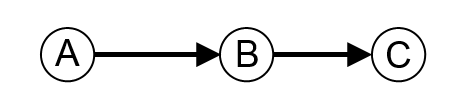
\includegraphics{images/dependency_graph_example.png}
    \caption{A simple example of a traditional dependency graph is shown. Here, node A's value depends on the value of node B, and node B's value depends on the value of node C.}
    \label{fig:dependency_graph_example}
\end{figure}

As such, this type of visualization lends itself well to illustrating the effect of causation in a system. Though causation can be difficult to determine in a complex system, as we have already shown, correlation is calculable via the PCC and other metrics, and a correlation-generalized undirected correlation graph could be envisioned, wherein two nodes have an undirected edge if their mutual PCC score exceeds a certain threshold, and have no edge if their mutual PCC score fails to meet that threshold. The steps to generate such a graph are as follows:

\begin{enumerate}
    \item At a given point in time, generate a PCC matrix for all of the possible data channel pairs.
    \item Generate an unconnected graph in which there exists a degree-0 node for each data channel.
    \item For node-node pair, add a connecting edge if there exists a PCC score above a reasonably high correlation threshold (e.g., $r_{PCC}^{2} > 0.8$). This edge can be colored to show correlation sign (e.g., blue for $r_{PCC} < 0$ and red for $r_{PCC} > 0$).
    \item Finally, cull all nodes that are still of degree 0.
\end{enumerate}

With the corrgram visualization, we needed to illustrate all possible pairs of channels as a separate cell, and thus ended up needing to visualize $\frac{n!}{2 (n - 2)!}$ different cells (where $n$ is the number of data channels). However, with a dependency graph visualization, we can reduce the number of colored elements (nodes) to a count of $n$, by introducing connecting edges. (For systems that are not highly correlated, this will produce far less visual clutter than the corrgram visualization.) Furthermore, we can simplify the undirected dependency graph visualization by eliminating any components of degree 0, if the correlated components are the only ones we wish to see.

We experimented with actually creating this visualization for explorational purposes. First, we ran a system dynamics simulation for our lunar rover described in Chapter 5. We paused the telemetry analysis at a certain time step at which interesting correlated components were present, and examined the data channel correlations at that instant. The correlated components are illustrated in the correlation map visualization in Fig.~\ref{fig:comparison_correlation_map}. We then isolated the correlated components and illustrated them as an undirected dependency graph, using the steps outlined above. The resulting undirected dependency graph visualization, with positive and negative correlation edges both visible, is shown in Fig.~\ref{fig:undirected_both}. In addition, positive and negative correlated components have been isolated into separate graphs for readability and discoverability, as shown in Fig.~\ref{fig:undirected_positive_only} and Fig.~\ref{fig:undirected_negative_only}, respectively.

\begin{figure}[h]
\centering
    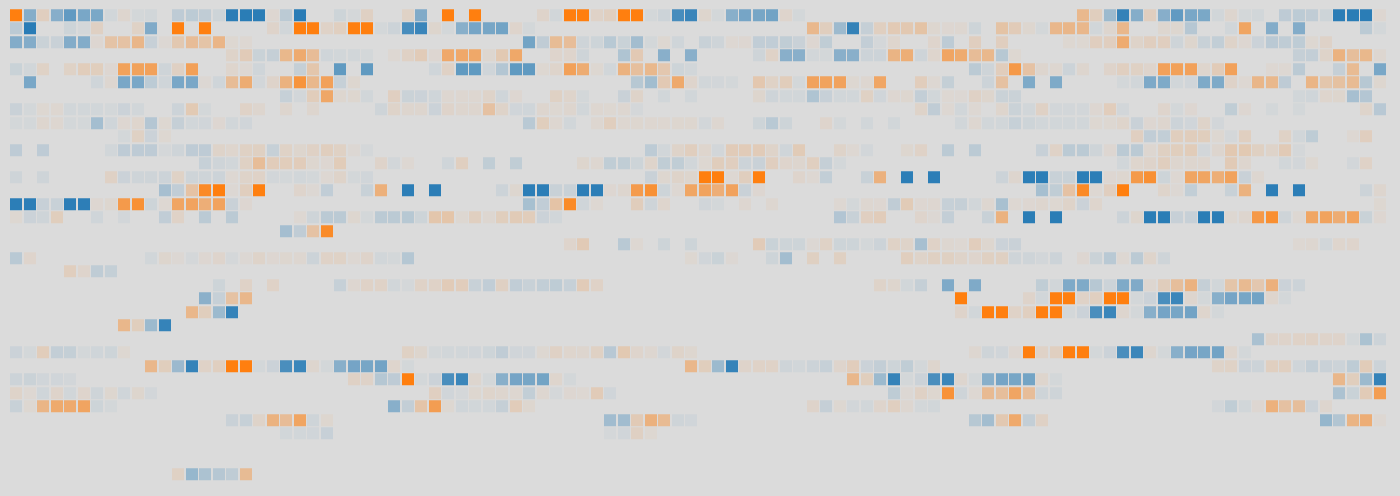
\includegraphics[width=\columnwidth]{images/comparison_correlation_map.png}
    \caption{A snapshot of the correlation map display from a simulated run. Note the strong correlations illustrated by opaque orange (positive) and blue (negative) cells.}
    \label{fig:comparison_correlation_map}
\end{figure}

\begin{figure}[h]
\centering
    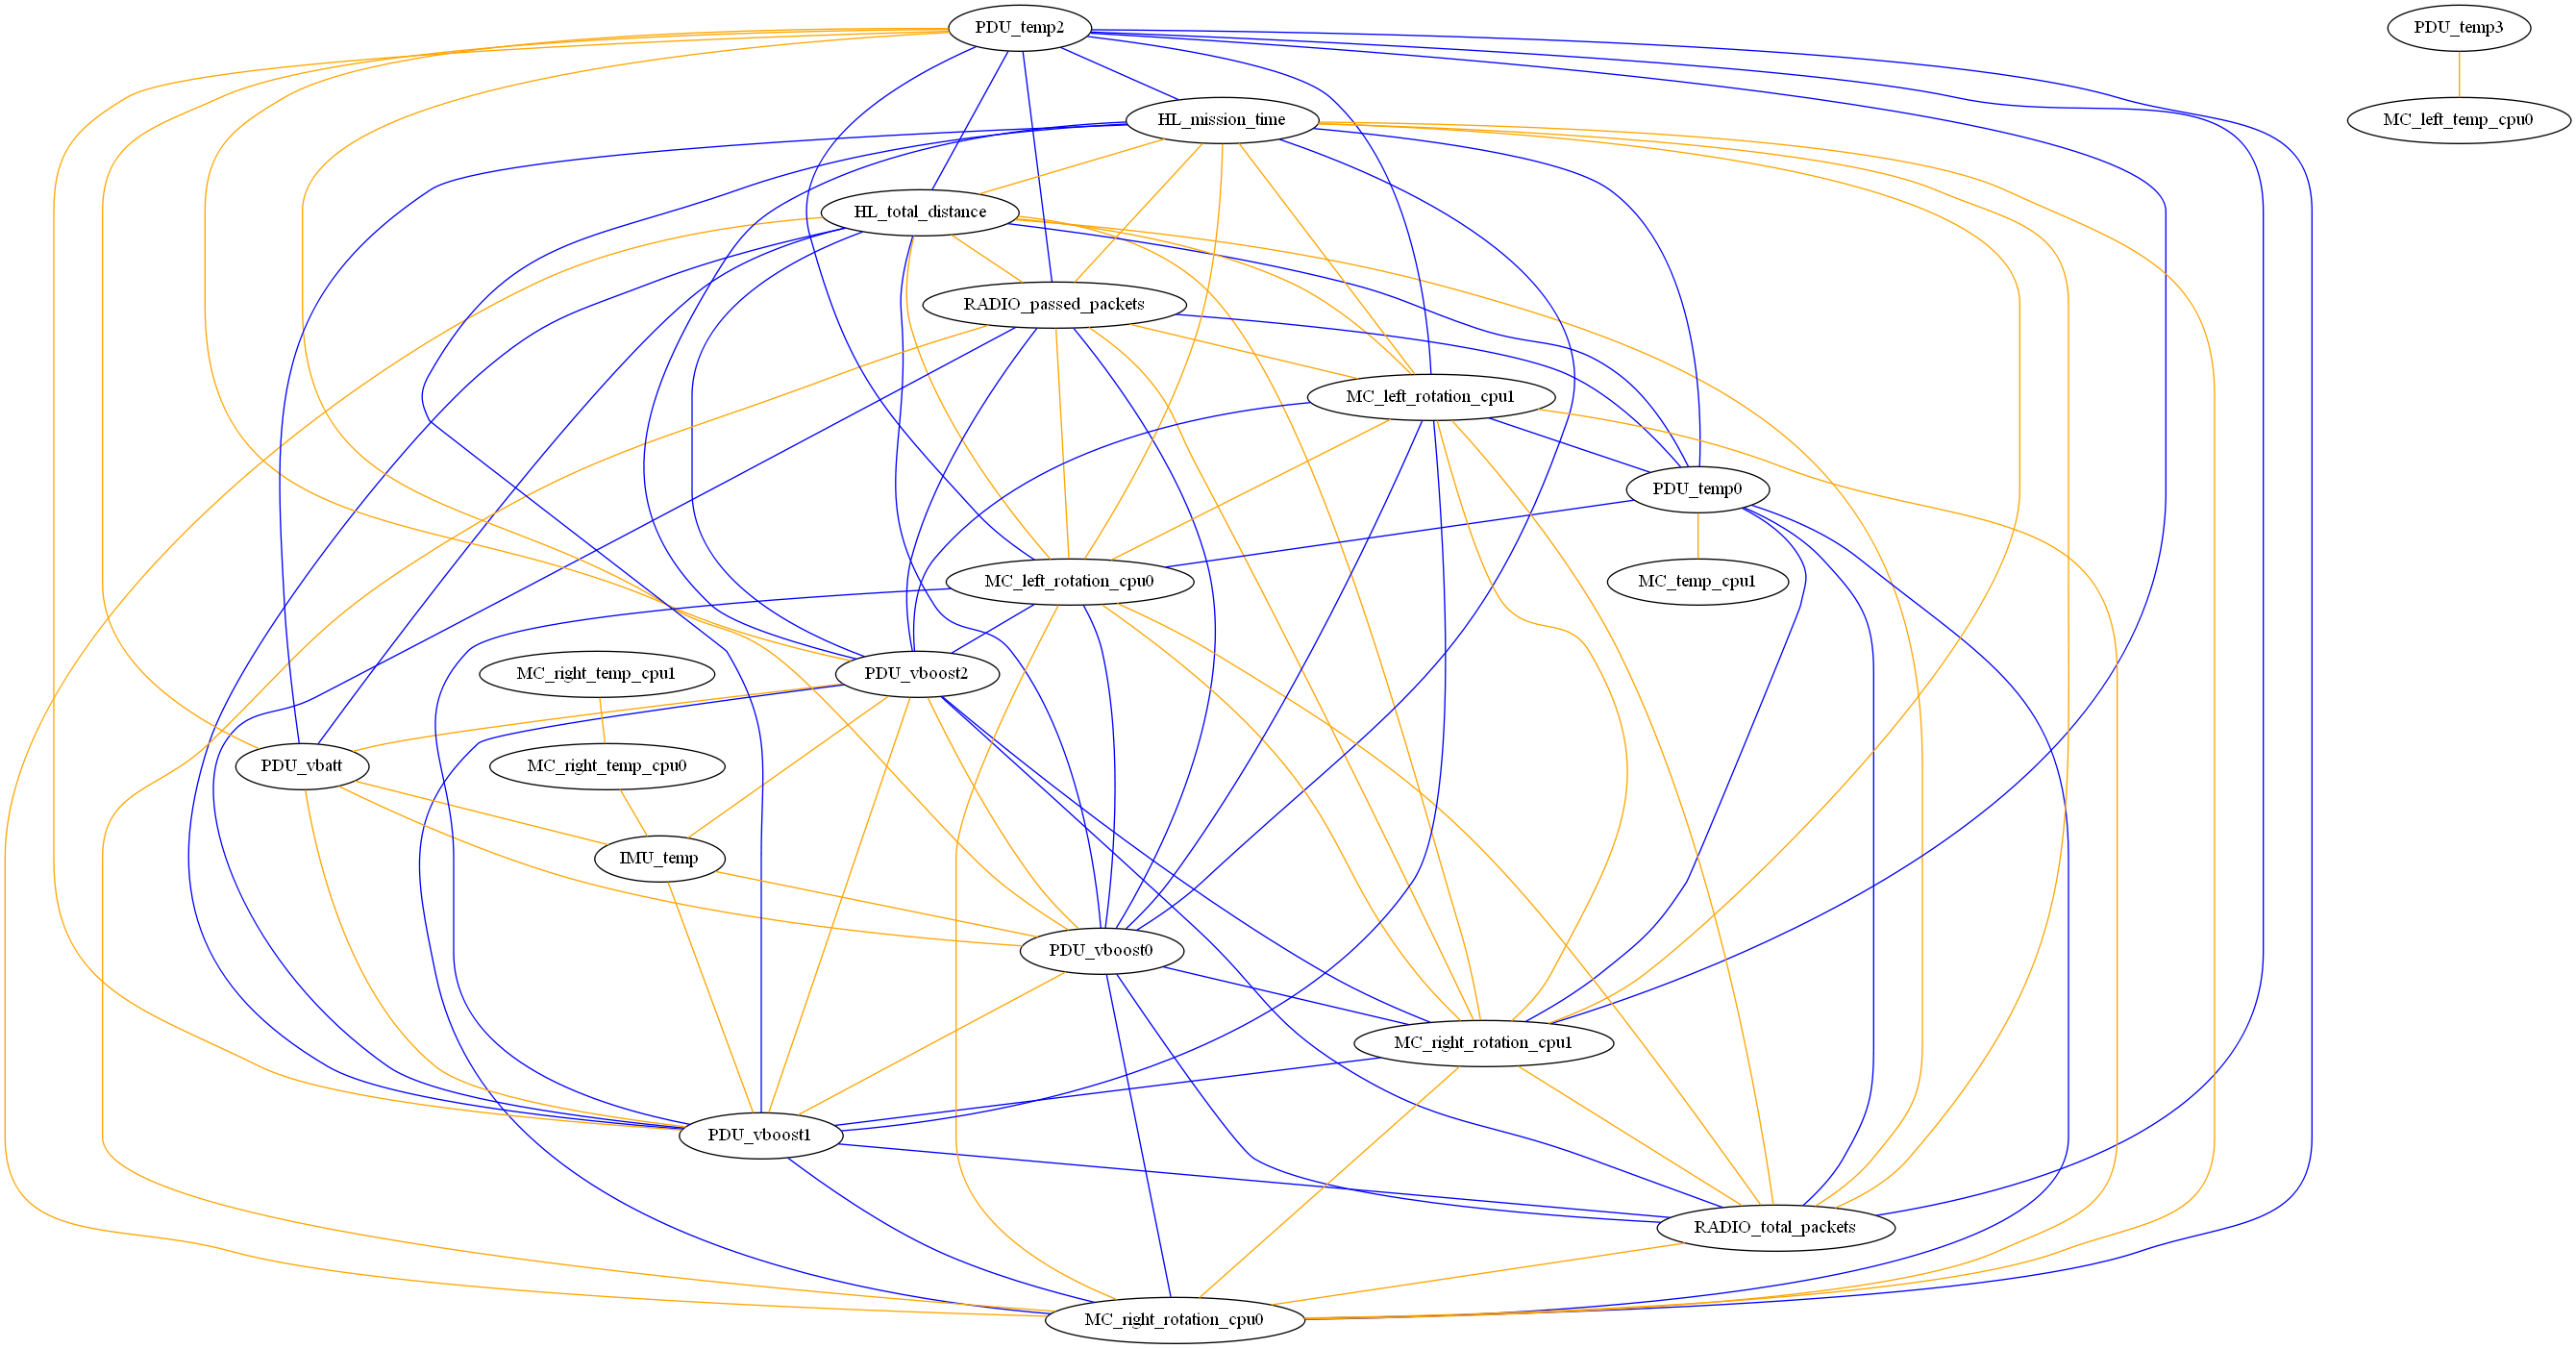
\includegraphics[width=\columnwidth]{images/undirected_both.png}
    \caption{A snapshot of an undirected dependency graph display from a simulated run. Correlated components have been isolated, with edges drawn for all correlation relationships exceeding a certain value ($r_{PCC}^{2} > 0.8$). Both positive and negative correlation connections are shown. Self-correlations are not shown.}
    \label{fig:undirected_both}
\end{figure}

\begin{figure}[h]
\centering
    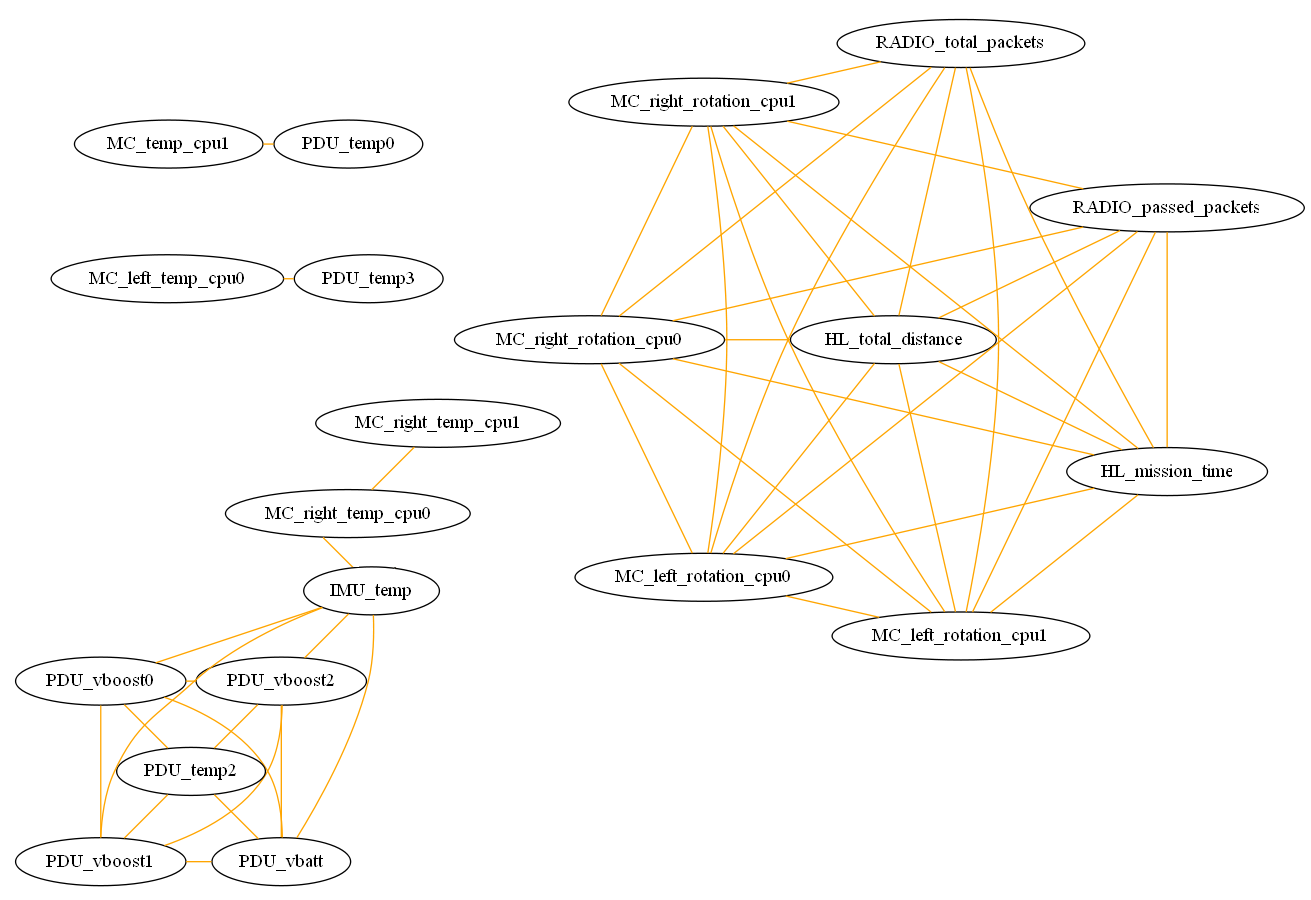
\includegraphics[width=\columnwidth]{images/undirected_positive_only.png}
    \caption{A snapshot of an undirected dependency graph display from a simulated run. Correlated components have been isolated, with edges drawn for all correlation relationships exceeding a certain value ($r_{PCC}^{2} > 0.8$). Only positive correlations are shown. Self-correlations are not shown.}
    \label{fig:undirected_positive_only}
\end{figure}

\begin{figure}[h]
\centering
    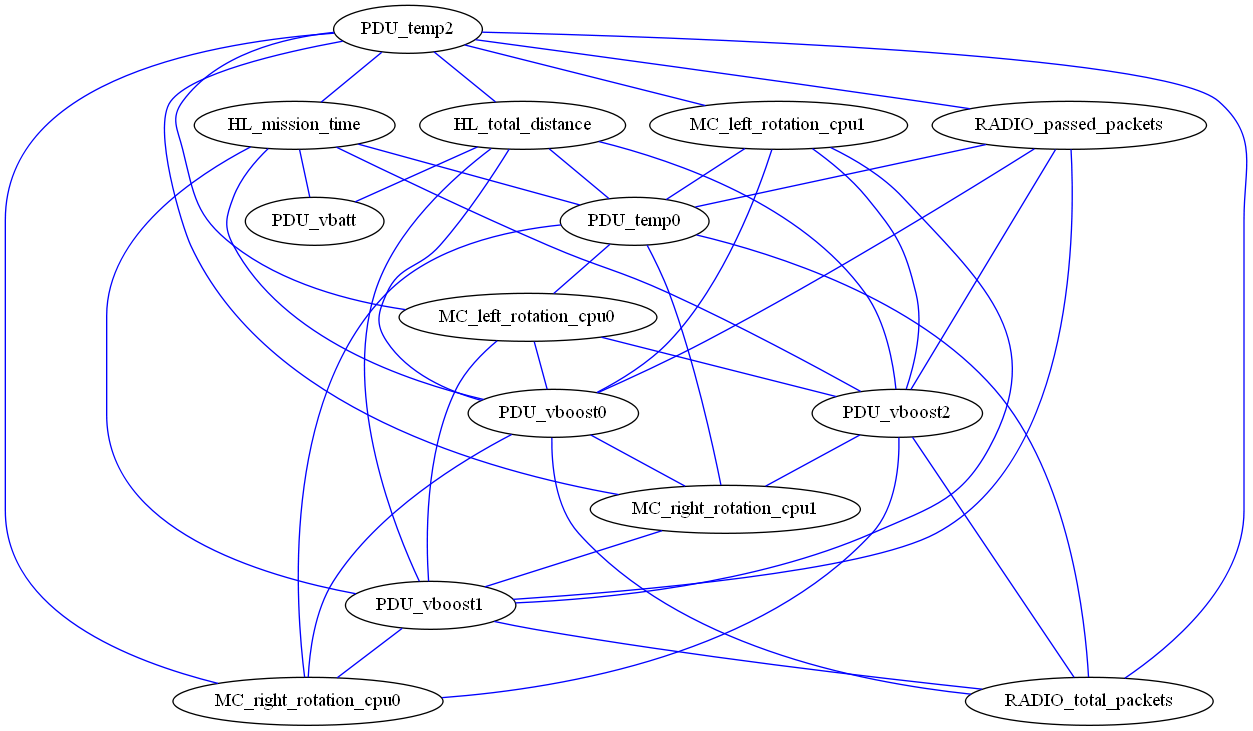
\includegraphics[width=\columnwidth]{images/undirected_negative_only.png}
    \caption{A snapshot of an undirected dependency graph display from a simulated run. Correlated components have been isolated, with edges drawn for all correlation relationships exceeding a certain value ($r_{PCC}^{2} > 0.8$). Only negative correlations are shown. Self-correlations are not shown.}
    \label{fig:undirected_negative_only}
\end{figure}

These visualizations present a very different way of viewing the correlative data. While the temporal dimension is still only captured as a snapshot (i.e., the correlative state at only one time point can be shown at a time), correlated components are shown very clearly, and can be understood at a glance. In particular, the intuition behind the positive correlated components in Fig.~\ref{fig:undirected_positive_only} seems clear; the most fully-connected, major clusters are exhibiting behavior which is very similar to each other. (In fact, the lower left cluster channels were all in a state of monotonic decrease, and the upper right cluster channels were in a state of monotonic increase.) The negative correlated components are less obvious, as they don't ``cluster" in the same way; however, the negative correlation data can be overlaid onto the positive correlation graphs as a higher-level operation on the clusters. This, perhaps, produces the most informative type of graph; this application is shown in Fig.~\ref{fig:undirected_positive_with_negative_clusters}.

Note that \cite{yeh2007exploratory} uses a similar approach for graph visualization of correlation matrices relationships; however, they impose a radial structure on all graph layouts, which losing the clustering advantage of the graph layouts we have produced here.

\begin{figure}[h]
\centering
    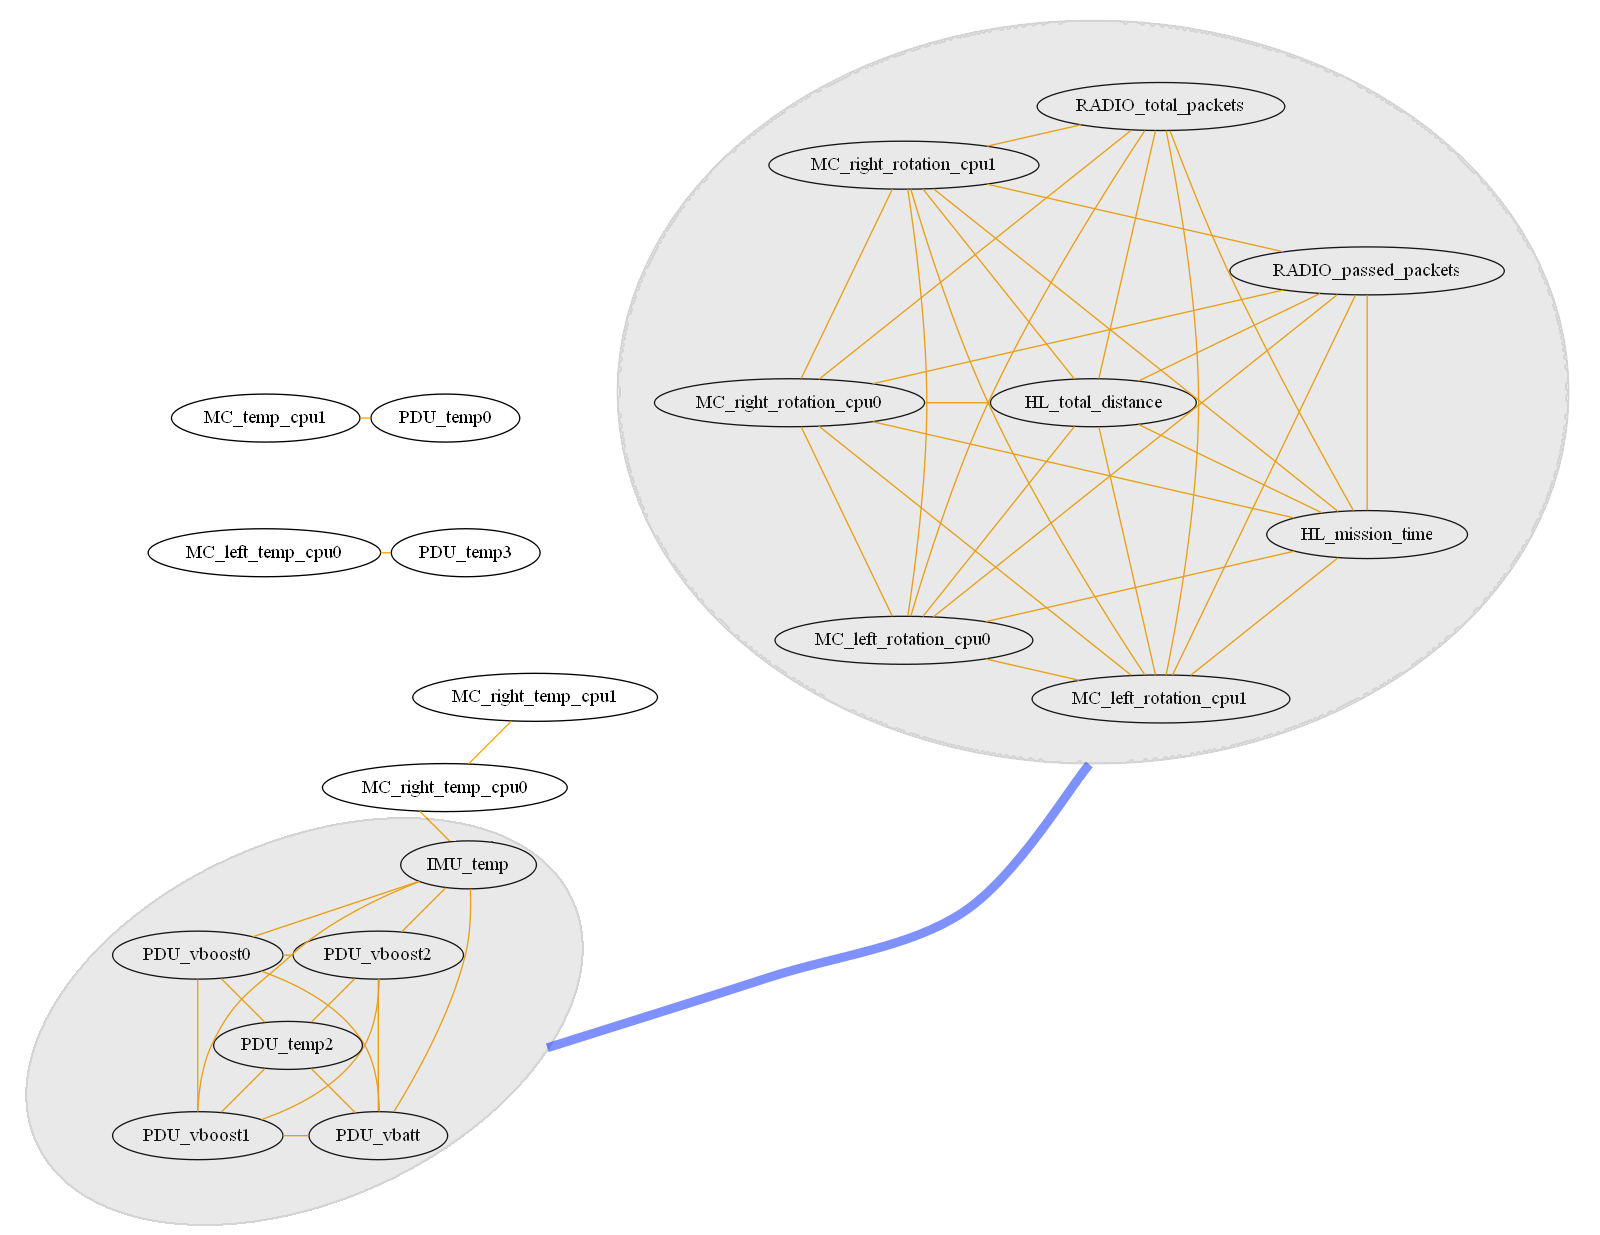
\includegraphics[width=\columnwidth]{images/undirected_positive_with_negative_clusters.png}
    \caption{A snapshot of an undirected dependency graph display from a simulated run. Correlated components have been isolated, with edges drawn for all correlation relationships exceeding a certain value ($r_{PCC}^{2} > 0.8$). Positive correlations, and negatively correlated subgraphs, are shown. Self-correlations are not shown.}
    \label{fig:undirected_positive_with_negative_clusters}
\end{figure}

Another advantage of this technique is that it clearly isolates small groups of correlated components; low-degree subgraphs can point towards noisy data, or towards significant links, but if they are persistent, it seems they may suggest interesting correlations that deviate from the patterns exhibiting by the bulk of the data channels, which tend to correlate due to behavior exhibiting positive and negative monotonicity. However, towards the idea of exploring a visualization which can show the evolution of state and correlative data over time, we will look at another technique in the following section.

\section{Time Curves}

In early 2016, Bach et al presented a powerful new type of visualization tool called ``Time Curves" \cite{bach2016time}. The time curve is a generic 2D embedding algorithm designed specifically for system state data which changes over time. Time curves visualize system states as a series of points, connected in temporal along curves within the 2D embedding. This allows the viewer to gain an understanding of system behavior by the shape and directions of the curves, and by the grouping of the data points. A visual example of how a time curve is ``folded" from an initial linear timeline is shown in Fig.~\ref{fig:time_curve_example}.

\begin{figure}[h]
\centering
    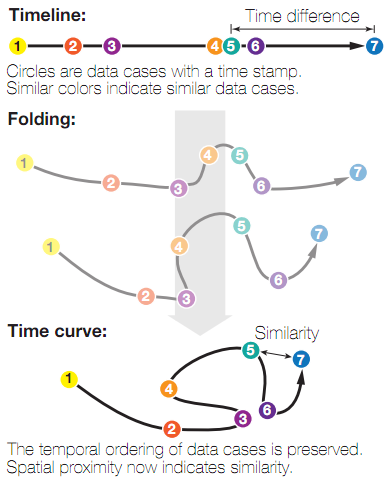
\includegraphics[width=0.5\columnwidth]{images/time_curve_example.png}
    \caption{A time curve is ``folded" from an initial linear timeline to bring similar data points close together in the 2D embedding. From \cite{bach2016time}.}
    \label{fig:time_curve_example}
\end{figure}

Let's take a closer look at how time curves model system behavior. In the time curves description, states over time are described as a series of ``time points," where each time point is a vector $\bar{x} \in \mathbb{R}^{n}$. For $t$ time points, the state at each time point can be horizontally packed into a matrix $M \in \mathbb{R}^{n \times t}$, which represents the full state history of the system.

The time curves algorithm uses a handful of multidimensional scaling (MDS) techniques which seek to map 2D Euclidean embedding distance to a user-supplied measure of vector distance, such that significantly ``similar" states are nearby in the embedding, while significantly ``different" states are far away in the embedding. The essential component to generating this embedding is the construction of a symmetric distance matrix $D \in \mathbb{R}^{t \times t}$, such that $D_{ij} = D_{ji}$ provides a pairwise distance score representing the difference between the states $M_{:,i}$ and $M_{:,j}$. A typical choice for this distance is a Euclidean norm, though many alternatives exist \cite{bach2016time}. The time curves algorithm performs an MDS optimization step to map the 2D embedding to the pairwise state distances described in $D$, producing the final visualization.

The time curves algorithm has many characteristics which make it an appealing candidate for complex system visualization. It exhibits \textbf{clustering}, where time points of similar states gather at very close points in the embedding. The viewer's eye naturally processes these clusters as single groups, and they may easily map to system modes. Time curves visualize \textbf{cycles}, where a time curve comes back to an earlier point in the embedding after moving elsewhere. This is very useful for modeling cyclic dynamics in complex systems. Time curves also emphasize \textbf{transitions} between clusters of points, as the embedding naturally pushes distinct clusters geometrically apart from each other.

Finally, time curves are very extensible, and can be combined with higher-level data which provides further insight into the state at a given time point.

\section{Applying Time Curves to System Telemetry Data}

We set about applying time curves to complex system telemetry data, in order to compare visualization results for raw state telemetry and correlative states, and to see if anomalous system modes could easily be identified in the resulting embeddings. Our data processing pipeline for raw state telemetry visualization was as follows:

\begin{enumerate}
    \item At regular intervals (e.g., once per second), record the telemetered system state into a vector $\bar{x} \in \mathbb{R}^{n}$.
    \item Once the mission is complete, horizontally concatenate all state vectors to produce a state history matrix $M \in \mathbb{R}^{n \times t}$.
    \item Generate a symmetric distance matrix $D \in \mathbb{R}^{t \times t}$, such that $D_{ij} = D_{ji}$ provides a pairwise distance score representing the difference between the states $M_{:,i}$ and $M_{:,j}$.
    \item Use the time curves algorithm to generate a 2D embedding of the $t$ states described in $D$.
\end{enumerate}

In contrast, our pipeline for generating visualizations for correlated telemetry was as follows:

\begin{enumerate}
    \item Generate a state history matrix $M$ as with the raw state telemetry case.
    \item For a given window size $w$, generate windowed ``sample matrices" $W \in \mathbb{R}^{n \times w}$, such that $W_{i} = M_{:, i:i+15}$.
    \item For each windowed matrix $W$, generate a correlative matrix $R \in \mathbb{R}^{n \times n}$ (via PCC, Spearman's Rho, or Kendall's Tau), such that $R_{ij}$ gives the correlation score of $W_{i,:}$ and $W_{j,:}$. (Note that incalculable correlations, such as those with data channels of zero variance, are set to be 0.)
    \item Flatten each windowed matrix $R$, and concatenate them horizontally into a matrix $C \in \mathbb{R}^{n^{2} \times (t - w)}$, such that each column of $C$ represents the total correlative state of the system at a time point.
    \item Generate a symmetric distance matrix $D \in \mathbb{R}^{(t - w) \times (t - w)}$, such that $D_{ij} = D_{ji}$ provides a pairwise distance score representing the difference between the states $C_{:,i}$ and $C_{:,j}$.
    \item Use the time curves algorithm to generate a 2D embedding of the $(t - w)$ states described in $D$.
\end{enumerate}

The algorithms described above were applied on the user testing data set used previously during user evaluations. This data set closely simulates telemetry from a lunar mission, in which the events described in Tbl.~\ref{tbl:events} take place at pre-set times. Each of these events triggers numerous differences in simulated environment state, which in turn causes major sensor data differences. High levels of Gaussian white noise have been introduced into the sensor data to approximate real sensor behavior.

The annotated time curve visualization of the raw state telemetry progression is shown in Fig.~\ref{fig:pfm2_raw_data_time_curve_annotated}. Similarly annotated visualizations of the PCC, Spearman's Rho, and Kendall's Tau correlative state are shown in Figs.~\ref{fig:pfm2_pcc_time_curve_annotated}, \ref{fig:pfm2_rho_time_curve_annotated}, and \ref{fig:pfm2_tau_time_curve_annotated}, respectively. (These correlative visualizations were generated with a 15-second time window.)

\section{Discussion}

The time curves visualization does a pleasing job of showing the varying modes of system operation, and allows the viewer to follow state progression easily. The major moves between groups of points correspond pretty much exactly to the times during the simulation when the rover started seeing telemetry differences from different environmental conditions.

It's also evident by inspection that the state progression from correlative analysis in Figs.~\ref{fig:pfm2_pcc_time_curve_annotated}, \ref{fig:pfm2_rho_time_curve_annotated}, and \ref{fig:pfm2_tau_time_curve_annotated} is more distinct and easy to understand than that visualized using raw telemetry in Fig.~\ref{fig:pfm2_raw_data_time_curve_annotated}. We believe that there are several reasons for these core differences. First, monotonically increasing data channels (e.g., time or wheel rotations) can make it hard to isolate modes, as state vectors containing this data appear to represent different states at each time step, even when they really only indicate one mode of behavior. These data channels can ``smear" the state across a 2D embedding, due to a steady, constant distance introduced through these increasing channels. Unless they are deliberately removed from the data--which could, as a side-effect, remove valuable data crucial to understanding system behavior--these data channels will result in behavior like that seen in Fig.~\ref{fig:pfm2_pcc_time_curve_annotated}, where the initial state and final state are actually very similar system modes, but are distint within the 2D embedding.

Additionally, changing environmental dynamics, and thus, the inputs into the system, can change as the environment changes, but if the vehicle continues to handle them in the same way, then the correlative relationships among its data channels may maintain more consistency in spite of these changing dynamics. Correlative analysis, in this way, allows a human operator to more directly investigate internal system relationships (although external dynamics still manifest themselves in the correlative data as correlations of sensor value behavior with time and other monotonically increasing values).

Finally, it appears that the correlative calculations, as they act on a large time window, appear to have had a denoising side-effect on the data, and allow real changes in correlation to clearly ``push" the time points around the embedding, making state transitions more clear--while state transitions within the raw telemetry visualization are subtle and mostly buried in the rest of the data.

Another interesting observation about the data produced, in particular visible within the correlative time curve visualizations, is the presence of additional states not foreseen in the event timeline, such as the cluster of time points between events \textbf{1} and \textbf{2}. Upon close analysis, this cluster of time points appears to be a ``hallucinated event," as a side-effect of several fault states being triggered at the same time and cascading effects on telemetered measurements as temperatures and generated voltages drop. The application of the PCC correlative algorithm emphasizes this state, likely because of its limitations with respect to accurately capturing nonlinear associations and the coarse, ordinal nature of a large amount of the discrete telemetry data.

\begin{table}[]
\centering
\begin{tabular}{lll}
Event Number & Timestamp & Event Description \\
0 & 0s & Rover begins traveling forward along smooth terrain. \\
1 & 188s & Rover enters crater; begins descending into crater. \\
2 & 287s & Rover enters shade, causing temp, comms, and power drops. \\
3 & 300s & Rover begins traversing smooth bottom of crater. \\
4 & 330s & Rover begins climbing out of crater. \\
5 & 343s & Rover exits shade; continues uphill. \\
6 & 534s & Rover emerges from crater and enters smooth terrain. \\
7 & 594s & Rover enters choppy terrain. \\
8 & 643s & Rover wheel has fault; rover stops moving.
\end{tabular}
\caption{Events during a visualized user simulation are shown. Cross-reference ``Event Numbers" with labels in Figs.~\ref{fig:pfm2_pcc_time_curve_annotated}, \ref{fig:pfm2_tau_time_curve_annotated}, \ref{fig:pfm2_rho_time_curve_annotated} and \ref{fig:pfm2_raw_data_time_curve_annotated} to see correspondence.}
\label{tbl:events}
\end{table}

\begin{figure}[h]
\centering
    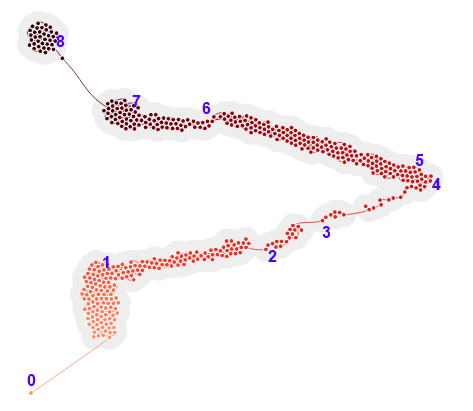
\includegraphics{images/pfm2_raw_data_time_curve_annotated.png}
    \caption{A time curve embedding visualizing mission events using raw telemetry state. Event annotations are described in Tbl.~\ref{tbl:events}.}
    \label{fig:pfm2_raw_data_time_curve_annotated}
\end{figure}

\begin{figure}[h]
\centering
    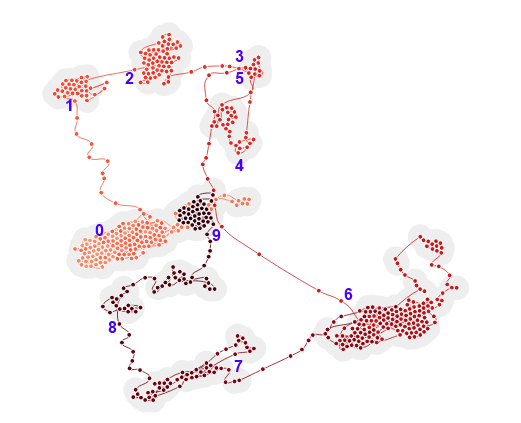
\includegraphics{images/pfm2_pcc_time_curve_annotated.png}
    \caption{A time curve embedding visualizing mission events using PCC correlation state. Event annotations are described in Tbl.~\ref{tbl:events}.}
    \label{fig:pfm2_pcc_time_curve_annotated}
\end{figure}

\begin{figure}[h]
\centering
    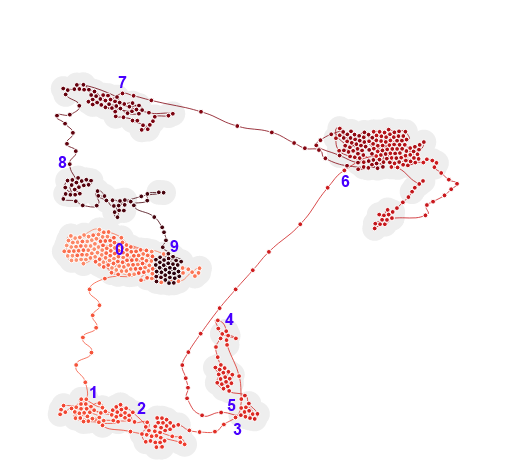
\includegraphics{images/pfm2_rho_time_curve_annotated.png}
    \caption{A time curve embedding visualizing mission events using Spearman's Rho correlation state. Event annotations are described in Tbl.~\ref{tbl:events}.}
    \label{fig:pfm2_rho_time_curve_annotated}
\end{figure}

\begin{figure}[h]
\centering
    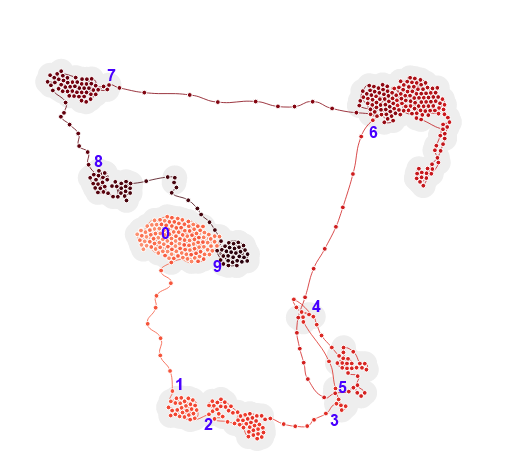
\includegraphics{images/pfm2_tau_time_curve_annotated.png}
    \caption{A time curve embedding visualizing mission events using Kendall's Tau correlation state. Event annotations are described in Tbl.~\ref{tbl:events}.}
    \label{fig:pfm2_tau_time_curve_annotated}
\end{figure} % Dimensional Reduction and Visualization Improvements

\chapter{Results and Discussion}

This chapter discusses the final results of our investigation into system analysis and visualization for fault diagnostic purposes.

\section{A Section}

Quisque tristique urna in lorem laoreet at laoreet quam congue. Donec dolor turpis, blandit non imperdiet aliquet, blandit et felis. In lorem nisi, pretium sit amet vestibulum sed, tempus et sem. Proin non ante turpis. Nulla imperdiet fringilla convallis. Vivamus vel bibendum nisl. Pellentesque justo lectus, molestie vel luctus sed, lobortis in libero. Nulla facilisi. Aliquam erat volutpat. Suspendisse vitae nunc nunc. Sed aliquet est suscipit sapien rhoncus non adipiscing nibh consequat. Aliquam metus urna, faucibus eu vulputate non, luctus eu justo.

\subsection{System State Visualization with Time Curves}


\section{Another Section}

Phasellus nisi quam, volutpat non ullamcorper eget, congue fringilla leo. Cras et erat et nibh placerat commodo id ornare est. Nulla facilisi. Aenean pulvinar scelerisque eros eget interdum. Nunc pulvinar magna ut felis varius in hendrerit dolor accumsan. Nunc pellentesque magna quis magna bibendum non laoreet erat tincidunt. Nulla facilisi.

Duis eget massa sem, gravida interdum ipsum. Nulla nunc nisl, hendrerit sit amet commodo vel, varius id tellus. Lorem ipsum dolor sit amet, consectetur adipiscing elit. Nunc ac dolor est. Suspendisse ultrices tincidunt metus eget accumsan. Nullam facilisis, justo vitae convallis sollicitudin, eros augue malesuada metus, nec sagittis diam nibh ut sapien. Duis blandit lectus vitae lorem aliquam nec euismod nisi volutpat. Vestibulum ornare dictum tortor, at faucibus justo tempor non. Nulla facilisi. Cras non massa nunc, eget euismod purus. Nunc metus ipsum, euismod a consectetur vel, hendrerit nec nunc. % Conclusion and Future Work

%% ----------------------------------------------------------------
% Now begin the Appendices, including them as separate files

\addtocontents{toc}{\vspace{2em}} % Add a gap in the Contents, for aesthetics

\appendix % Cue to tell LaTeX that the following 'chapters' are Appendices

\chapter{Relevant Code Samples}

This appendix contains a sampling of some of the most relevant code used to generate the results shown in this paper. Over 10,000 lines of code were written for this research, but only an illustrative subset of this code is shown here.

\section{Generating Example Corrgrams for PCC, Kendall's Tau, and Spearman's Rho Correlations (MATLAB)}

\lstinputlisting[language=Matlab]{code/basic_shaded_correlation_matrix_viz.m}

\section{Generating Undirected Graph from Filtered Correlation Data (Python)}

\lstinputlisting[language=Python]{code/gen_undirected_graph.py}

\section{Generating Time Curve Distance Matrix from Raw Telemetry (Python)}

\lstinputlisting[language=Python]{code/telem_csv_to_time_curves_format.py}

\section{Generating Correlated Distance Matrices from Bucketed Telemetry (MATLAB)}

\lstinputlisting[language=Matlab]{code/telem_to_correlation_to_timecurve_distance.m}	% Code Appendix

%\chapter{Usability Testing Script}\label{appendix:usability_test}


This appendix gives a detailed timeline of the usability tests performed for the Moonraker lunar rover, and gives the script read by the test coordinator during each of the tests.

\section{Approximate Simulated Run Timeline}

Users will be told that this is a straight-forward, long distance run. The run takes place on the Moon, towards the end of the lunar day. The cameras are non-functional for known (but irrelevant) reasons. 

\begin{itemize}

\item 0s: Mission start, commence driving forward (wheel telemetry, attitude changing normally), slow temperature gain from movement.
\item 188s: Rover starts moving slightly downhill, RSSI slowly degrades, chance of latency and packet drops increases.
\item Motor temperature gain drops due to downhill.
\item 287s: Battery charge voltage suddenly drops (in the shade). Temperature begins to fall on all systems.
\item 300s: Rover reaches bottom of crater floor, and travels along flat-ish ground for some time.
\item 330s: Rover starts moving uphill out of the crater. RSSI slowly increases, chance of latency and packet drops decreases. Motor temperature gain increases due to uphill.
\item 343s: Battery charge voltage suddenly increases (out of the shade). Temperature rising again on all systems.
\item 534s: Rover moves to flat ground again.
\item 594s: Attitude gets much choppier here (rough terrain).
\item 643s: Rover stops suddenly with motor fault (rock stuck in wheel).

\end{itemize}

\section{Test Script}

[Start script to send demo (non-test) telemetry to the rover]

Thanks for agreeing to test the Moonraker ground station interface. Note that this is a test of the software, not of you, so just relax and have fun.

In this test, you're a copilot for Moonraker. You're observing part of the lunar mission, and monitoring the telemetry, but you won't be sending any rover commands. Instead, you'll be looking for patterns in the data that indicate meaningful events, and explaining the story of these events.

This run is a long-distance, straight forward run on the Moon. The time is near the end of the lunar day. You won't be using the cameras. You can assume that they have stopped working for reasons that are understood, but which are not relevant to this run.

First, I'll do a quick overview of the data you can see. You have access to three screens.

This is the Pilot screen, which shows high-level data. Please click the Hakuto logo in the upper-left.

This is the Copilot screen, which shows lower-level data. Please click the Hakuto logo in the upper-left again.

This is the Correlation screen. This screen has a grid of squares, and each square shows the correlation between two channels of data. A correlation value of 1 indicates a strong positive correlation, -1 indicates a strong negative correlation, and 0 indicates no correlation.

You can switch between these three screens at any time by clicking the icon in the upper-left-hand corner of the screen. Feel free to use the screen which you feel gives you the most useful data at any given time.

Please go to the Pilot screen. Near the top is the Alert panel row, which tells you about the state of various sets of data. Clicking on the panels in this row will give you detailed information about what's happening with Moonraker.

In the lower-right of the Pilot screen, you can see controls to pause the incoming data to review it at any time. When paused, incoming data will continue to be received, but will not be shown until you unpause. Feel free to pause to review data at any time. You can also use the A, S, D, and F keys on the keyboard to manipulate data.

The run will take about 10 minutes, if you'd like to wait until the end of the run to pause, rewind, and review data, you're free to do so.

After the run is complete and the rover has stopped, I'd like you to try to develop a story for all of the events that happened. Once you're satisfied with your explanation story, please tell me what you think and what led you to those conclusions, and that will conclude the test. The time limit is 30 minutes.

Do you have any questions before we begin?

[Respond to any questions]

I will begin the test momentarily. As you monitor data, I'd like you to do a narrative outloud. What do you see? What is it telling you? What do you infer? What are you thinking? As much as possible, please think outloud for the entire test.

The test will now begin.

[Restart Unity editor; start script to send testing telemetry to the rover at 30 seconds mission time]

[Finished telling the story]

Do you have any general comments, thoughts, or suggestions?

[At the end of the test, thank them for their participation, and tell them not to discuss the details of this test with anyone until the end of the week.] % Appendix Title

%\input{Appendices/AppendixC} % Appendix Title

\addtocontents{toc}{\vspace{2em}}  % Add a gap in the Contents, for aesthetics
\backmatter

%% ----------------------------------------------------------------

\label{Bibliography}
\lhead{\emph{Bibliography}}  % Change the left side page header to "Bibliography"
\bibliographystyle{plain}  % Use the "unsrtnat" BibTeX style for formatting the Bibliography
\bibliography{bibliography}  % The references (bibliography) information are stored in the file named "Bibliography.bib"

\end{document}  % The End
%% ----------------------------------------------------------------